%!TEX root = ../main.tex

\chapter{Preliminary definitions} \label{chapt:preliminary-definitions}

In this chapter we introduce all concepts needed to understand the work of my thesis.

We start from the basics with \textit{B{\"u}chi Automata} and \textit{$\omega$-regular languages}. We mention them and explain two important classes of $\omega$-regular languages: SAFETY and coSAFETY.

We go on with \textit{Linear Temporal Logic} ($\ltl$) focusing on Extended Bounded Response LTL with past ($\ebrltl$), an enrichment of LTL with past temporal operators and bounded operators, that has the feature of being as expressive as the safety fragment of LTL.

Linear Temporal Logic and B{\"u}chi Automata are combined to verify LTL properties on models of systems. This technique is called \textit{Automaton-based LTL Model Checking} and is paired with \textit{Reduced Ordered Binary Decision Diagrams} (ROBDDs) to develop symbolic model checking that can cope with real-wold systems.
ROBDDs are a very popular data structure to manipulate efficiently boolean formulas. Representing B{\"u}chi Automata and Transitions Systems as boolean formulas, we can exploit ROBDDs to represent and manipulate set of states (regions) instead of explicit representations. 

% AIGER and SMV
During the thesis we have used a format to describe circuits and a language for the description of finite state systems. We are speaking of the \textit{AIGER format} and the \textit{SMV language}.

Finally, we introduce the \textit{Reactive Synthesis} problem, its game-theoretical formulation and the basic algorithms to solve it. Such basic algorithms can be enriched thanks to ROBDDs, so we present their symbolic formulations. We explain a technique to perform reactive synthesis from Extended Bounded Response LTL specifications.

%!TEX root = ../../main.tex

\section{B{\"u}chi Automata and \texorpdfstring{$\omega$}{omega}-regular languages}

Our journey starts with one of the formalism that more than others stands at the basis of computer science: Automata theory. 
Automata theory has a wide range of applications in various fields, including compiler design, robotics, artificial intelligence and cryptography. Above all, the field where automata fit perfectly is formal methods, in particular the model checking and reactive synthesis fields. For each type of automata we give the formal definition, the acceptance condition and the language describe by them.

The first type of automata we study are the ones over finite words belonging to an alphabet. 
NFAs and DFAs are automata over finite words and each automaton over finite words recognizes a language of finite words $\lang{} \subseteq \Sigma^*$.

\begin{definition}[\cite{intro-automata} Finite Automata (NFA and DFA)]
A Non-deterministic Finite Automata is a tuple $\automaton = \langle \Sigma, Q,I,\delta,F \rangle$, where: (i) $\Sigma$ is a finite alphabet; (ii) $Q$ is a finite set of states; (iii) $I \subseteq Q$ is the set of initial states; (iv) $\delta \subseteq Q \times \Sigma \times Q$ is the transition relation; (v) $F \subseteq Q$ is the set of final states. \\
If $\delta$ is a function $\delta \colon Q \times \Sigma \to Q$, we say that $\automaton$ is a Deterministic Finite Automata.
\end{definition}

\begin{definition}[\cite{intro-automata} Run and language of a NFA]
Let $\automaton = \langle \Sigma,Q,I,\delta,F \rangle$ be a NFA, and let $\sigma = \sequence{\sigma_0,\dots,\sigma_n} \in \Sigma^*$ be a finite word, for some $n \in \Nat$. 
A run of $\automaton$ over $\sigma$ is a finite sequence of states $\tau = \sequence{q_0,\dots q_{n+1}}$ such that $q_0 \in I$ and $\tuple{q_i,\sigma_i,q_{i+1}} \in \delta$, for each $i \in [0,n]$.
We say that $\tau$ is accepting if and only if its last state is a final state, that is $q_{n+1} \in F$.
A word $\sigma \in \Sigma^*$ is accepted by $\automaton$ if and only if there exist an accepting run of $\automaton$ over $\sigma$. The language accepted by $\automaton$, denoted as $\lang{(\automaton)}$, is the set of all and only the words $\sigma \in \Sigma^*$ accepted by $\automaton$.
\end{definition}

When we enter in the fields of model checking and reactive synthesis, NFAs are not enough anymore. That's because we want to verify a system and so deal with infinite executions, in order to classify them as either good or bad runs. Therefore, a more powerful formalism is required.
One of the first types of automata reading infinite words that were introduced is the class of B{\"u}chi automata, which were introduced to prove the decidability of the logic $S1S$ (the monadic second-order theory of $\Nat$ under successor) over infinite linear order \cite{B66}. 
In the following years thanks to the ability to accept infinite languages of infinite words, B{\"u}chi automata has been used to solve the LTL model checking problem \cite{VW86}.

As for the case of NFAs, B{\"u}chi Automata can be split in Non-determistic B{\"u}chi Automata and Deterministic B{\"u}chi Automata. NBAs differ from NFAs from the acceptance condition. Since B{\"u}chi Automata must cope with infinite words, an infinite word is accepted if and only if the set of final states is visited infinitely many times. 

\begin{definition}[\cite{wolgang-1991} $\omega$-word and $\omega$-language]
Let $\Sigma$ be a finite alphabet. An \textit{infinite word} (or $\omega$-word) over $\sigma$ is simply an infinite sequence $\sigma_0,\sigma_1,\dots$ where each $\sigma_i \in \Sigma$. We denote with $\Sigma^\omega$ the set of all infinite words over the alphabet $\Sigma$.
We say that $\omegalang{}$ is a $\omega$-language if $\omegalang{} \subseteq \Sigma^\omega$
\end{definition}

\begin{definition}[\cite{wolgang-1991} B{\"u}chi Automata (NBA and DBA)]
A Non-deterministic B{\"u}chi Automata (NBA) is a tuple $\automaton = \tuple{\Sigma,Q,I,\delta,F}$, where: (i) $\Sigma$ is a finite alphabet; (ii) $Q$ is a finite set of states; (iii) $I \subseteq Q$ is the set of initial states; (iv) $\delta \subseteq Q \times \Sigma \times Q$ is the transition relation; (v) $F \subseteq Q$ is the set of acceptance states.
If $\delta$ is a function $\delta \colon Q \times \Sigma \to Q$, we say that $\automaton$ is a \textit{Deterministic B{\"u}chi Automata}.
\end{definition}

\begin{definition}[\cite{wolgang-1991} Run and Language of a NBA]
Let $\automaton = \tuple{\Sigma,Q,I,\sigma,F}$ be a NBA and $\sigma = \sequence{\sigma_0,\sigma_1} \in \Sigma^{w}$ be a $\omega$-word over $\Sigma$.
A run of $\automaton$ over $\sigma$ is an infinite sequence of states $\tau = \sequence{q_0,q_1,\dots} \in Q^w$ such that $q_0 \in I$ and $\tuple{q_i,\sigma_i,q_{i+1}} \in \delta$, for each $i \in [0,n]$.
We say that $\tau$ is accepting if and only if $q_i \in F$ for infinitely many $i \in \Nat$.
A $\omega$-word $\sigma$ is accepted by $\automaton$ if and only if there exist an accepting run of $\automaton$ over $\sigma$. 
The language accepted by $\automaton$, denoted as $\omegalang{(\automaton)}$, is the set of all and only the $\omega$-words $\sigma \in \Sigma^\omega$ accepted by $\automaton$.
\end{definition}

In contrast with NFA and DFA, where for every NFA $\automaton$ there exists an DFA automaton $\automaton'$ such that $\lang{(\automaton)} = \lang{(\automaton')}$, some NBA that cannot be converted to an equivalent DBA.

NBAs recognize $\omega$-regular languages, that is languages obtained from $\omega$-regular expressions (sequence obtained from symbols in $\Sigma$ and basic operations, union, concatenation and repetition). Since the aim of my thesis is not investigating $\omega$-languages, I would prefer not introducing $\omega$-regular languages formally, but them as the class of languages recognize by NBAs. $\omega$-regular languages are closed under all Boolean operations. 
An example of NBA can be found in \autoref{fig:nba-example}, where the double-circle state is the accepting one.

\begin{theorem}[\cite{cf-automata} $\omega$-regular language]
Given a $\omega$-language $\omegalang{}'$, we say that $\omegalang{}'$ is $\omega$-regular if and only if there exists a NBA $\automaton$ which accepts all $\omega$-words in the language.
In particular, we have that $\omegalang{}' = \omegalang{(\automaton)}$.
We denote the class of $\omega$-regular languages as $\omega$-REG.
\end{theorem}

\begin{figure}[!htp]
    \centering
    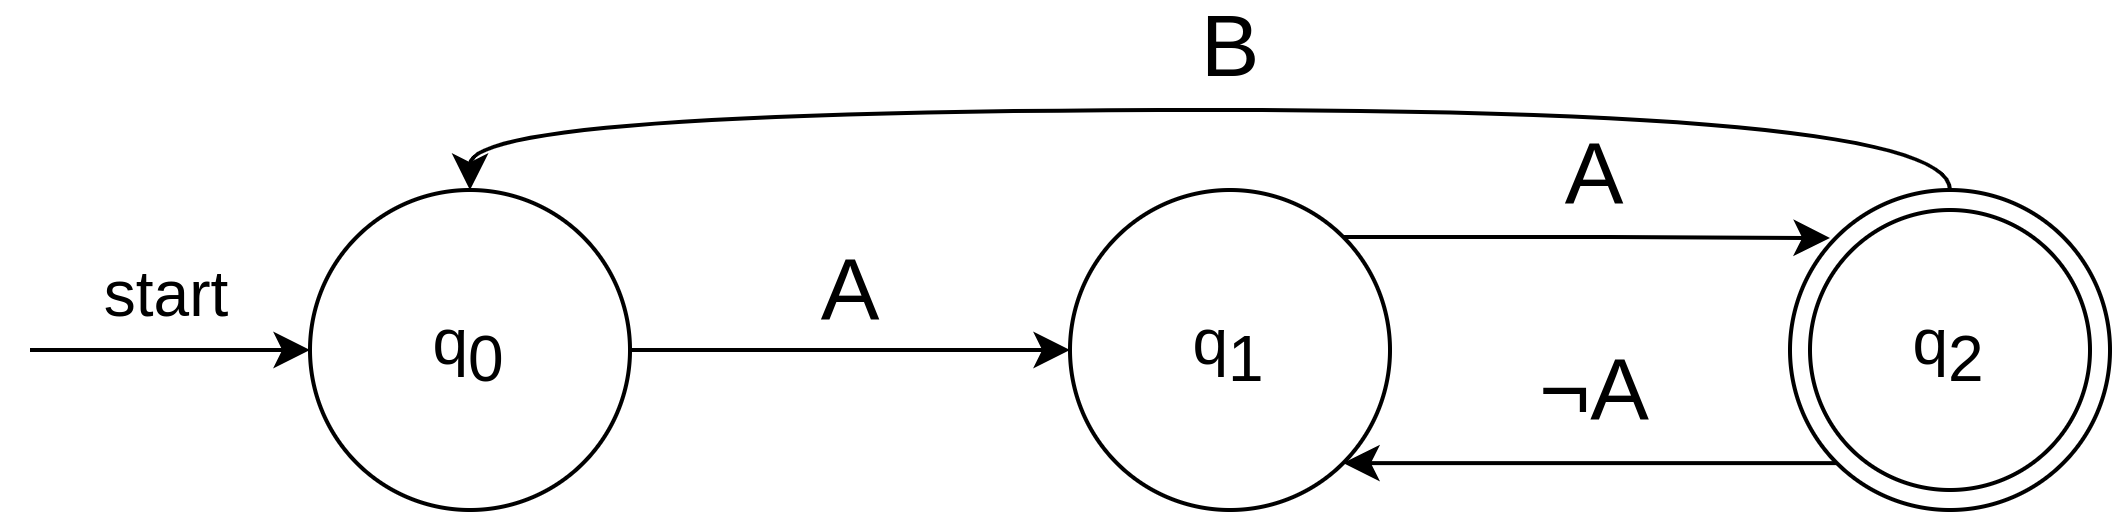
\includegraphics[width=0.8\linewidth]{figures/nba-example.png}
    \caption{Example of NBA accepting any word where every B is preceded by a positive even number of A}
    \label{fig:nba-example}
\end{figure}

There exists a generalization of B{\"u}chi Automata with $n$ acceptance sets of states and the acceptance condition changes as follows: there exists some states that visit each acceptance set of states infinitely many times. It is always possible to compile a Generalized B{\"u}chi Automaton to a Non-deterministic B{\"u}chi Automaton, but GBAs are easier to be used in many cases, like some model checking algorithms.

\begin{definition}[\cite{gastin-oddoux-2001} Generalized B{\"u}chi Automata (GBA)]
A Generalized B{\"u}chi Automata $\automaton$ is a tuple $\automaton = \tuple{\Sigma,Q,I,\delta,\set{F_1,\dots,F_n}}$ where $\Sigma$, $Q$, $I$ and $\delta$ have the same definition of a NBA, but there are $n$ acceptance sets of states $F_1,\dots,F_n$ such that $F_i \subseteq Q$ for all $i \in [1,n]$.
\end{definition}

\begin{definition}[\cite{gastin-oddoux-2001} Run and Language of a GBA]
Let $\automaton = \tuple{\Sigma,Q,I,\sigma,\set{F_1,\dots,F_n}}$ be a GBA and $\sigma = \sequence{\sigma_0,\sigma_1} \in \Sigma^{w}$ be a $\omega$-word over $\Sigma$.
A run of $\automaton$ over $\sigma$ is an infinite sequence of states $\tau = \sequence{q_0,q_1,\dots} \in Q^w$ such that $q_0 \in I$ and $\tuple{q_i,\sigma_i,q_{i+1}} \in \delta$, for each $i \in [0,n]$.
We say that $\tau$ is accepting if and only if for each acceptance set of states $F \in \set{F_1,\dots,F_n}$ there exists a state $q_i \in F$ for infinitely many $i \in \Nat$.
A $\omega$-word $\sigma$ is accepted by $\automaton$ if and only if there exist an accepting run of $\automaton$ over $\sigma$. 
The language accepted by $\automaton$, denoted as $\lang{\automaton}$, is the set of all and only the $\omega$-words $\sigma \in \Sigma^\omega$ accepted by $\automaton$.
\end{definition}

Two important classes of $\omega$-regular languages comprise those languages that express the fact that something bad never happens, called safety languages, and those languages that express that fact that something good eventually happens, called co-safety languages.
The class of the $\omega$-regular co-safety languages coSAFETY is defined as the dual of SAFETY, that is the set of languages $\omegalang{}$ such that $\omegalang{} \in coSAFETY$ iff $\bar{\omegalang{}} \in SAFETY$, where $\bar{\omegalang{}}$ is the complement language of $\omegalang{}$.

\begin{definition}[\cite{geatti-2021-09} Safety languages]
Let $\omegalang{} \subseteq \Sigma^\omega$ be an $\omega$-regular language. We say that $\omegalang{}$ is a safety language if and only if for all words $\sigma \in \Sigma^\omega$ it holds that, if $\sigma \not\in \lang{}$, then $\exists i \in \Nat .\; \forall \sigma' \in \Sigma^\omega .\; \sigma_{[0,i]} \cdot \sigma' \not\in \lang{}$. We call $\sigma_{[0,i]}$ a bad-prefix since it leads to a state where a word can not be in the language no matter how it is going to evolve.
The class of safety $\omega$-regular languages is denoted as SAFETY.
\end{definition}

\begin{definition}[\cite{geatti-2021-09} Co-safety languages]
Let $\omegalang{} \subseteq \Sigma^\omega$ be a $\omega$-regular language. We say that $\omegalang{}$ is a co-safety language if and only if for all words $\sigma \in \Sigma^\omega$ it holds that, if $\sigma \in \lang{}$, then $\exists i \in \Nat .\; \forall \sigma' \in \Sigma^\omega .\; \sigma_{[0,i]} \cdot \sigma' \in \lang{}$. We call $\sigma_{[0,i]}$ a good-prefix since it leads to a state where a word is in the language no matter how it is going to evolve.
The class of co-safety $\omega$-regular languages is denoted as coSAFETY.
\end{definition}

Since each $\omega$-regular language is recognized by a NBA, it is easy to see that we could categorize all automata accepting safety languages. This type of automata is called Safety Automata and are used a lot in my thesis, so let me state them.

\begin{definition}[\cite{gastin-oddoux-2001} Safety Automata (NSA and DSA)]
A Non-deterministic Safety Automata is a tuple $\automaton = \tuple{\Sigma,Q,I,\delta}$, where: (i) $\Sigma$ is a finite alphabet; (ii) $Q$ is a finite set of states; (iii) $I \subseteq Q$ is the set of initial states; (iv) $\delta \subseteq Q \times \Sigma \times Q$ is the transition relation.
If $\delta$ is a partial function $\delta \colon Q \times \Sigma \to Q$, we say that $\automaton$ is a Deterministic Safety Automata (NSA). 
\end{definition}

\begin{definition}[\cite{gastin-oddoux-2001} Run and Language of a NSA]
Let $\automaton = \tuple{\Sigma,Q,I,\sigma}$ be a NSA and $\sigma = \sequence{\sigma_0,\sigma_1} \in \Sigma^{w}$ be a $\omega$-word over $\Sigma$.
A run of $\automaton$ over $\sigma$ is an infinite sequence of states $\tau = \sequence{q_0,q_1,\dots} \in Q^w$ such that $q_0 \in I$ and $\tuple{q_i,\sigma_i,q_{i+1}} \in \delta$, for each $i \in [0,n]$.
A $\omega$-word $\sigma$ is accepted by $\automaton$ if and only if there exist a run of $\automaton$ over $\sigma$. 
The language accepted by $\automaton$, denoted as $\omegalang{(\automaton)}$, is the set of all and only the $\omega$-words $\sigma \in \Sigma^\omega$ accepted by $\automaton$.
\end{definition}

It is simple to see that the language recognized by any safety automaton is a safety language, since the only way for a $\omega$-word to be rejected by a safety automaton is to induce a run that at some point gets stuck, i.e. it can not continue to any state reading the current letter. This implies that a $\omega$-word rejected by a safety automaton is rejected in a finite number of steps, inducing a bad-prefix.  

\begin{theorem}
Given $\omegalang{}$ a language over infinite words, $\omegalang{} \in SAFETY$ if and only if $\omegalang{}$ is recognized by some NSA.
\end{theorem}

%!TEX root = ../../main.tex

\section{Linear Temporal Logic}

After a brief introduction to B{\"u}chi Automata and $\omega$-regular languages, concede us to jump to the logic world with Linear Temporal Logic.

Linear Temporal Logic ($\ltl$) is a modal logic interpreted over infinite, discrete and linear ordered time. $\ltl$ can be seen as an extension of propositional logic with the addition of the \textit{next} operator ($\ltlX{\phi}$, i.e. at the next state $\phi$ holds) and the \textit{until} operator ($\ltlU{\phi_1}{\phi_2}$, i.e. $\phi_2$ will eventually hold and $\phi_1$ will hold until then).

\begin{definition}[\cite{geatti-2021-09} The logic $\ltl$]
Let $\Sigma$ be a set of propositions, $\ltl$ formulas are inductively defined as follows:
\begin{flalign*}
\phi := p \; | \; \ltlNeg{\phi} \; | \;  \ltlOr{\phi_1}{\phi_2} \; | \; \ltlX{\phi} \; | \; \ltlU{\phi_1}{\phi_2}
\end{flalign*}
where $p \in \Sigma$.
\end{definition}

Linear temporal logic with Past ($\pastltl$) extends $\ltl$ with the addition of temporal operators that can talk about the past, and it is obtained from $\ltl$ by adding the following past temporal operators: the $\textit{yesterday}$ operator ($\ltlY{\phi}$, i.e. there exists a previous state in which $\phi$ holds); the \textit{weak yesterday} operator ($\ltlZ{\phi}$, i.e. either a previous state does not exist or in the previous state $\phi$ holds); the \textit{since} operator ($\ltlS{\phi_1}{\phi_2}$, i.e. there was a past state where $\phi_2$ held and $\phi_1$ has held since then). 

\begin{definition}[ \cite{geatti-2021-09} The logic $LTL+P$]
Let $\Sigma$ be a set of propositions, $LTL+P$ formulas are inductively defined as follows:
\begin{flalign*}
\phi := p \; &| \; \ltlNeg{\phi} \; | \;  \ltlOr{\phi_1}{\phi_2} \; | \; \ltlAnd{\phi_1}{\phi_2}
\tag{propositional connectives}\\
&|\; \ltlX{\phi} \; | \; \ltlU{\phi_1}{\phi_2} \;
\tag{future temporal operators} \\
&| \; \ltlY{\phi} \; | \; \ltlZ{\phi} \; | \; \ltlS{\phi_1}{\phi_2}
\tag{past temporal operators} \\
\end{flalign*}
where $p \in \Sigma$.
\end{definition}

To simplify writing of formulas, we define following abbreviations:
\begin{enumerate}[label=\roman*.]
    \item true: $\ltlTrue \equiv \ltlOr{\phi}{\ltlNeg{\phi}}$; false: $\ltlFalse \equiv \ltlAnd{\phi}{\ltlNeg{\phi}}$; implication: $\ltlImpl{\phi_1}{\phi_2} \equiv \ltlOr{\ltlNeg{\phi_1}}{\phi_2}$; iff: $\ltlIff{\phi_1}{\phi_2} \equiv \ltlAnd{\ltlImpl{\phi_1}{\phi_2}}{\ltlImpl{\phi_2}{\phi_1}}$;
    \item $\ltlXexp{\phi}{i}$ is $\ltlX{\ltlXexp{\phi}{i-1}}$ if $i > 0$ and $\phi$ if $i=0$;
    \item release: $\ltlR{\phi_1}{\phi_2} \equiv \ltlNeg{(\ltlU{\ltlNeg{\phi_1}}{\ltlNeg{\phi_2}})}$, i.e. either $\phi_2$ is always true, or it will happen that $\phi_1$ is true and in the meantime $\phi_2$ is always true; 
    \item eventually: $\ltlF{\phi} \equiv \ltlU{T}{\phi}$, i.e. $\phi$ will be true eventually;
    \item globally: $\ltlG{\phi} \equiv \ltlNeg{\ltlF{\ltlNeg{\phi}}}$, or $\ltlG{\phi} \equiv \ltlR{\ltlFalse}{\phi}$, i.e. $\phi$ is always true;
    \item trigger: $\ltlT{\phi_1}{\phi_2} \equiv \ltlNeg{(\ltlS{\ltlNeg{\phi_1}}{\ltlNeg{\phi_2}})}$, i.e. either $\phi_2$ was always true in the past, or it is happened that $\phi_1$ was true and in the meantime $\phi_2$ was always true;
    \item once: $\ltlO{\phi} \equiv \ltlS{\ltlTrue}{\phi}$, i.e. $\phi$ was true at least one time in the past; 
    \item historically: $\ltlH{\phi} \equiv \ltlNeg{\ltlO{\ltlNeg{\phi}}}$, i.e. $\phi$ was always true in the past.
\end{enumerate}

We can even make a further distinction starting from $\pastltl$. We say that a $\pastltl$ formula is \textit{pure past} if and only if all temporal operators inside the formula are past operators.
\textit{Full Past LTL} ($\fpltl$) is the fragment of $LTL+P$ that only admits past operators.

Formulas from $\pastltl$ are interpreted over state sequences. A \textit{state sequence} $\sigma = \sequence{\sigma_0,\sigma_1,\dots}$ is an infinite, linearly ordered sequence of states, where each state $\sigma_i$ is a set of proposition letters, that is $\sigma_i \in 2^\Sigma$ for $i \in \Nat$. Given two indices $i,j \in \Nat$ with $i \leq j$, we denote as $\sigma_{[i,j]}$ the interval of $\sigma$ from index $i$ to $j$, that is $\langle \sigma_i,\dots,\sigma_j \rangle$.

To be more precise, let us formalize the semantics of temporal operators we have seen so far plus some additional abbreviations.

\begin{definition}[\cite{geatti-2021-09} $\pastltl$ semantics]
A state-sequence is an infinite sequence $\sigma = \sequence{\sigma_0,\sigma_1,\dots} \in (2^\Sigma)^\omega$ of sets of propositions $\sigma_i \in 2^\Sigma$.
Given a sequence $\sigma$, a position $i\geq 0$ and a formula $\phi$, the satisfaction of $\phi$ by $\sigma$ at $i$, written $\sigma,i \models \phi$, is inductively defined as follows:
\begin{flalign*}
&\sigma,i \models p             &\iff& & & p \in \sigma_i \\
&\sigma,i \models \ltlNeg{\phi} &\iff& & & \sigma,i \not\models \phi \\
&\sigma,i \models \ltlOr{\phi_1}{\phi_2} &\iff& & & \text{$\sigma,i \models \phi_1$ or $\sigma,i \models \phi_2$} \\
&\sigma,i \models \ltlAnd{\phi_1}{\phi_2} &\iff& & & \text{$\sigma,i \models \phi_1$ and $\sigma,i \models \phi_2$} \\
&\sigma,i \models \ltlX{\phi} &\iff& & & \sigma,i+1 \models \phi \\
&\sigma,i \models \ltlY{\phi} &\iff& & & \text{$i>0$ and $\sigma,i-1 \models \phi$} \\
&\sigma,i \models \ltlZ{\phi} &\iff& & & \text{$i=0$ or $\sigma,i-1 \models \phi$} \\
&\sigma,i \models \ltlU{\phi_1}{\phi_2} &\iff& & & \text{$\exists j \geq i$ such that $\sigma,j \models \phi_2$ and} \\
& & & & & \text{$\sigma,k\models \phi_1$ for all $i \leq k < j$} \\
&\sigma,i \models \ltlR{\phi_1}{\phi_2} &\iff& & & \text{either for all $j \geq i$ such that $\sigma,j \models \phi_2$,} \\
& & & & & \text{or $\exists j \geq i$ such that $\sigma,j \models \phi_1$ and} \\
& & & & & \text{$\sigma,k\models \phi_1$ for all $i \leq k \leq j$} \\
&\sigma,i \models \ltlS{\phi_1}{\phi_2} &\iff&&& \text{$\exists j \leq i$ such that $\sigma,j \models \phi_2$ and} \\
& & & & & \text{$\sigma,k\models \phi_1$ for all $j < k \leq i$}
\end{flalign*}
\end{definition}

We say that $\sigma$ satisfies $\phi$, written $\sigma \models \phi$, if and only if $\sigma,0 \models \phi$. In this case we call $\sigma$ a model of $\phi$.

$\ltl$ can also be enriched with bounded temporal operators, such as the \textit{bounded until} $\ltlUbounded{\phi_1}{\phi_2}{[a,b]}$, \textit{bounded eventually} $\ltlFbounded{\phi}{[a,b]} \equiv \ltlUbounded{\ltlTrue}{\phi_2}{[a,b]}$ and \textit{bounded globally} $\ltlGbounded{\phi}{[a,b]} \equiv \ltlNeg{\ltlFbounded{\ltlNeg{\phi}}{[a,b]}}$. We define the bounded until operator as a shortcut for the $\ltl$ formula $\bigvee_{i=a}^{b}(\ltlXexp{\psi_2}{i}\land \bigwedge_{j=0}^{i-1}\ltlXexp{\psi_1}{j})$.
\textit{Full Bounded LTL} ($\fbltl$) is the fragment of LTL that includes only the next and bounded eventually operators.

\textit{Extended Bounded Response LTL} ($\ebrltl$) extends $LTL_{FB}$ by admitting Boolean combinations of the universal unbounded temporal operators release ($\ltlR{}{}$) and globally ($\ltlG{}$).
If we allow using past operators in $\ebrltl$, then we get the $\pastebrltl$ which is defined as follows.

\begin{definition}[\cite{geatti-2020-08} The logic $\ebrltl$]
Let $a,b \in \Nat$. A $\ebrltl$ formula $\chi$ is inductively defined as follows:
\begin{flalign}
&\psi := p \; | \; 
        \ltlNeg{\psi} \; | \; 
        \ltlOr{\psi_1}{\psi_2} \; | \; 
        \ltlX{\psi} \; | \;
        \ltlUbounded{\psi_1}{\psi_2}{[a,b]}
        \tag{Bounded Future Layer} \\
&\phi := \psi \; | \; 
        \ltlAnd{\phi_1}{\phi_2} \; | \; 
        \ltlX{\phi} \; | \; 
        \ltlG{\phi} \; | \; 
        \ltlR{\psi}{\phi}
        \tag{Future Layer} \\
&\chi := \phi \; | \; 
        \ltlOr{\chi_1}{\chi_2} \; | \; 
        \ltlAnd{\chi_1}{\chi_2}
        \tag{Boolean Layer}
\end{flalign}
\end{definition}


\begin{definition}[\cite{geatti-2021-09} The logic $\pastebrltl$]
Let $a,b \in \Nat$, a $\pastebrltl$ formula $\chi$ is inductively defined as follows:
\begin{flalign}
&\eta := p \; | \; 
        \ltlNeg{\eta} \; | \;
        \ltlOr{\eta_1}{\eta_2} \; | \;
        \ltlY{\eta} \; | \;
        \ltlS{\eta_1}{\eta_2}
        \tag{Pure Past Layer} \\
&\psi := \eta \; | \; 
        \ltlNeg{\psi} \; | \; 
        \ltlOr{\psi_1}{\psi_2} \; | \; 
        \ltlX{\psi} \; | \;
        \ltlUbounded{\psi_1}{\psi_2}{[a,b]}
        \tag{Bounded Future Layer} \\
&\phi := \psi \; | \; 
        \ltlAnd{\phi_1}{\phi_2} \; | \; 
        \ltlX{\phi} \; | \; 
        \ltlG{\phi} \; | \; 
        \ltlR{\psi}{\phi}
        \tag{Future Layer} \\
&\chi := \phi \; | \; 
        \ltlOr{\chi_1}{\chi_2} \; | \; 
        \ltlAnd{\chi_1}{\chi_2}
        \tag{Boolean Layer}
\end{flalign}
\end{definition}

Before arguing the advantage to add past temporal operators to $\ebrltl$, we introduce the expressiveness of a temporal logic.
The notion of expressiveness of a temporal logic is an extension of the notion of equivalence of formulas.
We say that two formulas $\phi$ and $\psi$ are equivalent ($\phi \equiv \psi$) if and only if they are satisfied by the same set of state sequences.
A temporal logic $\logic$ is said to be at least as expressive as another temporal logic $\logic'$, if for each formula $\phi \in \logic$, there exists a formula $\psi \in \logic'$ such that $\phi \equiv \psi$.
A temporal logic $\logic$ is said to be less expressive than another temporal logic $\logic'$ if, there exists a formula $\phi \in \logic'$ that for each formula $\psi \in \logic$, $\phi \not\equiv \psi$.
Two temporal logic are equally expressive when they are at least as expressive as each other.

In \cite{geatti-2021-09} has been proved that, without past temporal operators, $\ebrltl$ is less expressive than the safety fragment of $\ltl$. However, we achieve the same expressiveness of the safety fragment of $\ltl$ by adding past temporal operators, becoming a safety language at the same level of other more famous LTL dialects, like $\ltlG{\alpha}$, i.e. formulas starting with \textit{globally} and ending with $\alpha$ is a \textit{pure past formula}, and \textit{Safety-LTL}, i.e. formulas of $\ltl$ without \textit{until} temporal operator and in Negation Normal Form (NNF).
Just to give the general idea of the proof of $\semantics{\ebrltl} \subsetneq \semantics{\ltl} \cap SAFETY$, we can show that the formula $\phi_G := \ltlG{(\ltlOr{p_1}{\ltlG{p_2}})}$ belongs syntactically to Safety-LTL, but it is not expressible by any $\ebrltl$ formula. On the contrary, note that $\phi_G$ is expressible in $\pastebrltl$ since $\phi_G := \ltlG{(\ltlOr{p_1}{\ltlG{p_2}})} \equiv \ltlG{(\ltlImpl{\ltlNeg{p_2}}{\ltlH{p_1}})}$.

\begin{theorem}[\cite{geatti-2021-09} Expressiveness of $\ebrltl$]
$\semantics{\ebrltl} \subsetneq \semantics{\ltl} \cap SAFETY$
\end{theorem}

\begin{theorem}[\cite{geatti-2021-09} Expressiveness of $\pastebrltl$]
$\semantics{\pastebrltl} = \semantics{\ltlG{\alpha}} = \semantics{\text{\textit{Safety-LTL}}} =  \semantics{\ltl} \cap SAFETY$
\end{theorem}

\subsection{Temporal Hierarchy}
Safety and Co-safety properties covers only a subset of all properties expressible by Linear Temporal Logic.
LTL formulas can be divided in classes that form a hierarchy, highlighting the relation among their normal forms defined as Boolean and temporal combinations of full-past formulas. For this reason, whenever we write $\alpha_1$, $\alpha_2$ in this sub-section, we mean two full-past formulas ($\alpha_1,\alpha_2 \in \fpltl$).
Such hierarchy is called Temporal Hierarchy and it was introduced by Manna and Pnueli \cite{pnueli1990}.

Previously we have seen two important type of classes, which are at base of the hierarchy: safety and co-safety properties. 
Safety properties express the fact that "something bad will never happen". An important type of safety properties are invariant properties, which are boolean propositions that must always hold. 
Safety properties are expressible by full-past formulas preceded by a globally operator ($\ltlG{\alpha}$).
Co-safety properties the fact that "a good thing will happen at least one time" and they are expressible by full-past formulas preceded by an eventually operator ($\ltlF{\alpha}$).

The next class of $\ltl$ properties is called obligation class and consists in Boolean combinations of the two classes defined above. 
Its name derived from the fact that its properties impose a conditional obligation ($\ltlOr{\ltlG{\alpha_1}}{\ltlF{\alpha_2}} \equiv \ltlImpl{\ltlF{\alpha_1'}}{\ltlF{\alpha_2}}$ with $\alpha_1' \equiv \ltlNeg{\alpha_1}$), where if something happens, then something else will happen. The normal form of the obligation class is the set of formulas of type $\bigwedge_{i=1}^n(\ltlOr{\ltlG{\alpha_1}}{\ltlF{\alpha_2}})$ for some $n \in \Nat$.

Another formulation for the previous class is the intersection of two other important classes: liveness and persistence. 
\textit{Liveness} expresses properties of type "a good thing will happen infinitely many times" and they are described by formulas of type $\ltlG{\ltlF{\alpha}}$. 
\textit{Persistence} expresses properties of type "a good thing will constantly happen from a certain point on and they are described by formulas of type $\ltlF{\ltlG{\alpha}}$.

Considering the Boolean combinations of liveness and persistence properties, we end up with the reactivity class. A \textit{reactivity} property, like an obligation property, expresses a conditional obligation of the type "if a good thing happens infinitely many times, so does another thing". The normal form of this class comprises all formulas of type $\bigwedge_{i=1}^{n}(\ltlOr{\ltlG{\ltlF{\alpha_1}}}{\ltlF{\ltlG{\alpha_2}}})$, expressible also as $\ltlImpl{\ltlG{\ltlF{\alpha_2'}}}{\ltlG{\ltlF{\alpha_1}}}$ with $\alpha_2' \equiv \ltlNeg{\alpha_2}$, for some $n \in \Nat$. Reactivity class is exactly the set of all $\ltl$ formulas and so they have the same expressiveness.
Actually, there is an entire hierarchy inside the reactivity class, where we define $R(n)$ for some $n \in \Nat$ as the classes of formulas with a fixed number $n$ of conjunctions.
Moreover, it is been proved that $\semantics{R(n)} \subsetneq \semantics{R(n+1)}$ for each $n \in \Nat$.


\begin{figure}[!htp]
    \centering
    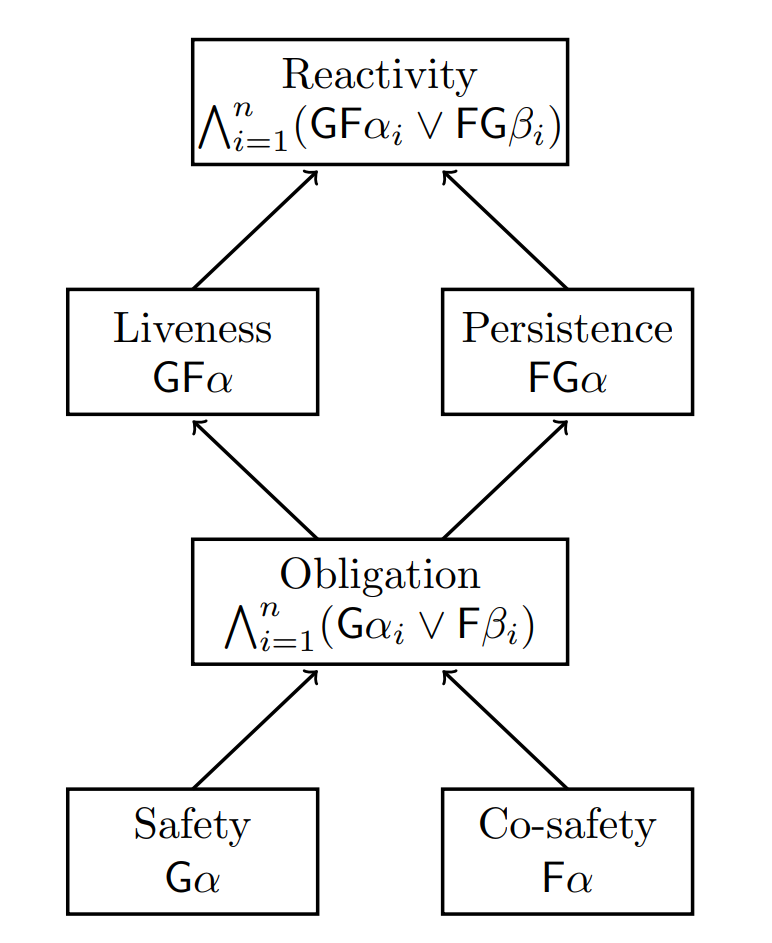
\includegraphics[width=0.4\linewidth]{figures/temporal-hierarchy.png}
    \caption{\cite{pnueli1990} Temporal Hierarchy describing the relation among temporal classes along with their normal forms. The arrows represent the inclusions between the classes.}
    \label{fig:temporal-hierarchy}
\end{figure}

%!TEX root = ../../main.tex

\section{Automaton-based LTL Model Checking}
\label{sec:ltl-model-checking}

In this section we merge B{\"u}chi automata and Linear Temporal Logic, presenting what an abstraction of a system is, the basic idea of Automaton-based LTL Model Checking and some useful definitions for later.
Automaton-based LTL Model Checking is the technique to verify a property $\phi$ expressed in $\ltl$ on a model of a system introduced for the first time by \cite{VW86}. 

Given a system, a model represents an abstraction of it. 
The model of a system is designed as a Transition System (TS), which is a mathematical model to describe the potential behaviour of discrete systems. It consists of states and transitions between states, which may be labeled with labels chosen from a set.
Transition Systems differ from finite-state automata in several ways: the set of states is not necessarily finite, the set of transitions is not necessarily finite and no start and final states are given. 
The most widely used type of Transition Systems is Labeled Transition Systems, which consists of Transition System with an additional labelling function mapping each node with a word over an alphabet $AP$.

Another way to design the model of a system is by Moore Machine or Mealy Machine. Both machines are finite-state machines, but differently from other finite automata that determine the acceptance of a particular string in a given language, they determine the output against given input. The formalization of the two machines is quite the same: a set of states, an initial state, input and output alphabets, a transition function and an output function. They differ only in the output function: in Mealy Machine the output function value depends on the current state and the current input symbol, while in Moore Machine the output function value depends only on the current state.

In this section we use LTS as main model, but we wanted to give the definition of Moore Machine and Mealy Machine since we are going to cite them in later chapters.

\begin{definition}[\cite{principles-cps} Labeled Transition System (LTS)]
A Labeled Transition System is a tuple $\model = \tuple{S, \to, I, AP, L}$ consisting of: (i) a finite set $S$ of states; (ii) a transition relation $\to \subseteq S \times S$; (iii) a set $I \subseteq S$ of initial states; (iv) a set $AP$ of atomic propositions (alphabet); (v) a labeling function $L \colon S \to 2^{AP}$.
\end{definition}

\begin{definition}[\cite{principles-cps} Moore Machine]
A Moore Machine is a tuple $\model = \tuple{S,s_0,I,O,\delta,\lambda}$ consisting of: (i) a finite set $S$ of states; (ii) an initial state $s_0 \in S$; (iii) a finite set called input alphabet; (iv) a finite set called output alphabet; (v) a transition function $\delta \colon S \times I \to S$; (vi) an output function $\lambda \colon S \to O$.
\end{definition}

\begin{definition}[\cite{principles-cps} Mealy Machine]
A Mealy Machine is a tuple $\model = \tuple{S,s_0,I,O,\delta,\lambda}$ consisting of: (i) a finite set $S$ of states; (ii) an initial state $s_0 \in S$; (iii) a finite set called input alphabet; (iv) a finite set called output alphabet; (v) a transition function $\delta \colon S \times I \to S$; (vi) an output function $\lambda \colon S \times I \to O$.
\end{definition}

From a set $s$ in a transition system we can define: the set of direct successors, i.e. the states reachable in one step; the set of direct predecessors, i.e. the states from which $s$ can be reached by one step; the set of states reachable by an undefined number of steps; the set of states from which $s$ can be reached by an undefined number of states; the set of states reachable starting from the initial states.

\begin{definition}[\cite{principles-cps} $Pre$, $Post$ and $reachability$ sets]
Let $\model = \tuple{S, \to, I, AP, L}$ be a Labeled Transition System and a state $s \in S$.
\begin{itemize}
    \item The set $Post(s)$ of direct successors of $s$ is defined by $Post(s) = \set{s' \in S \; | \; s \to s'}$.
    \item The set $Pre(s)$ of direct predecessors of $s$ is defined by $Pre(s) = \set{s' \in S \; | \; s' \to s}$.
    \item The set $Post^*(s)$ consists of the states reachable in the state graph from $s$. Given $C \subseteq S$, the set $Post^*(C)$ is defined by $Post^*(C) = \bigcup_{s \in C} Post^*(s)$.
    \item The set $Pre^*(s)$ consists of the states reachable in the state graph from $s$. Given $C \subseteq S$, the set $Pre^*(C)$ is defined by $Pre^*(C) = \bigcup_{s \in C} Pre^*(s)$.
    \item The set $Reach(TS) = Post^*(I)$ is the reachability set of TS from $I$.
\end{itemize}
\end{definition}

\begin{definition}[\cite{principles-cps} Paths and Traces sets]
Let $\model = \tuple{S, \to, I, AP, L}$ be a Labeled Transition System. 
\begin{itemize}
    \item A finite path fragment is a finite state sequence $\sequence{s_0,s_1,\dots,s_n}$ for some $n\geq 0$ such that $s_i \in Post(s_{i-1})$ for all $i < 0 \leq n$.
    \item An infinite path fragment is an infinite state sequence $\sequence{s_0,s_1,\dots}$ such that $s_i \in Post(s_{i-1})$ for all $i > 0$.
    \item A path fragment is initial if $s_0 \in I$. 
    \item The set $Paths(\model)$ defines all the initial paths of $\model$.
    \item A trace of an infinite path fragment is the sequence of sets of atomic propositions $\sequence{L(s_0), L(s_1), \dots} \in Traces(TS)$.
    \item The set $Traces(\model)$ defines all traces of all paths in $Paths(\model)$.
\end{itemize}
\end{definition}

After having described what a model of a system is, let us go on speaking about properties of a model. 
Given a model $\model$, we want to specify admissible traces. 
This can be done exploiting linear-time (LT) property over the atomic propositions $AP$, that is a subset of $(2^{AP})^\omega$. 
Since linear-time properties are hard to describe, we may need of a logic to describe them in a fancier way. 
Here $\ltl$ comes in play, because it is a logic allowing to describe linear time properties over the atomic proposition $AP$. 
When we speak about linear-time property via $\ltl$, it is useful recognizing the set of words described by $\phi$.

\begin{definition}[\cite{principles-cps} Words of a $\ltl$ formula]
Let $\phi$ be a $\ltl$ formula over $AP$, the set $Words(\phi)$ is defined as all the words where $\phi$ holds, i.e. $Words(\phi) = \set{\sigma \in (2^{AP})^\omega \; | \; \sigma \models \phi}$.
\end{definition}

LTL Model Checking is the task to say whether a formula $\phi$ is satisfied by a model $\model$. If that is case, then yes must be returned, otherwise a counterexample must be returned as the proof of $\model \not\models \phi$.
The underlying idea under Automaton-based LTL Model Checking is to verify whether all traces of $\model$ are subset of word of $\phi$, namely $\model \models \phi \iff Traces(TS) \subseteq Words(\phi)$. 
That is because we can say that $\model \models \phi$ only if $\phi$ holds no matter the trace undertaken by any execution of $\model$. 
Starting from this idea we deduce that we could reason even in a different way, that is there is no path on which the negation of $\phi$ holds. 
If such path exists, then it is a counterexample for $\model \models \phi$.
From here we can also do a next step. Now we are speaking about traces and words, but we can do the same reasoning speaking about automata.
Actually, for each $\ltl$ formula $\phi$ there exists a related automaton such that the language of $\phi$ and the language of such automaton are the same. 
This can be done by converting $\phi$ into a Generalized B{\"u}chi Automaton and then into a Non-deterministic B{\"u}chi Automaton. 
This unlocks the possibility to express the problem using automata. 
To perform Automaton-based LTL Model Checking we need to follow these steps:
\begin{itemize}
    \item construct the B{\"u}chi Automaton $\automaton_{\ltlNeg{\phi}}$ corresponding to the negated specification;
    \item build the product automaton between $\model$ and $\automaton_{\ltlNeg{\phi}}$;
    \item search for accepting cycles in the composition $\model \times \automaton_{\ltlNeg{\phi}}$. If there exists one cycle, then it means that $\ltlNeg{\phi}$ is satisfied, otherwise it means that $\phi$ is satisfied. In other words, we look for a point in the time from which is not possible to visit accepting states infinitely often.
\end{itemize}
Following we can see all previous concepts formally.

\begin{definition}[\cite{principles-cps} Counterexample]
A counterexample $\pi$ of a $\ltl$ formula $\phi$ over a LTS $\model$ is a path (even infinite) such that $\pi \not\models \phi$.
\end{definition}

\begin{theorem}[\cite{VW86}]
For any $\ltl$ formula $\phi$ over $AP$, there exists a NBA $\automaton_{\phi}$ over $2^{AP}$ such that $Words(\phi) = \omegalang{(\automaton_{\phi})}$.
\end{theorem}

\begin{definition}[\cite{principles-cps} Product automaton between LTS and NBA]
Let $\model = \tuple{S, \to, I, AP, L}$ be a LTS and $\automaton = \tuple{Q,\Sigma,\delta,Q_0,F}$ with $\Sigma = 2^{AP}$ and $Q_0 \cap F = \emptyset$. Their product is defined as the transition system $\model \times \automaton = \tuple{S',\to',I',AP',L'}$ where: 
\begin{enumerate}[label=\roman*.]
    \item $S' = S \times Q$;
    \item $\to'$ is defined by 
    \[ \infer{s \to t \land q \xrightarrow{L(t)} p}{\tuple{s,q} \to' \tuple{t,p}} \]
    \item $I' = \set{\tuple{s_0, q} \; | \; s_0 \in I \land \exists q_0 \in Q_0 \; : \; q_0 \xrightarrow{L(s_0)} q}$;
    \item $AP' = Q$; 
    \item $L' \colon S \times Q \to 2^Q$ with $L'(\tuple{s,q}) = {q}$.
\end{enumerate}
\end{definition}

\begin{definition}[Automaton-based $\ltl$ model checking]
We say that $\model$ satisfies $\phi$, denoted as $\model \models \phi$, if for each path $\pi$ of $\model$ it holds that $\pi \models \phi$, i.e. if $Traces(\model) \subseteq Words(\phi)$.
Equivalently, $\model \models \phi$ if and only if there does not exist a path $\pi$ such that $\model \models \ltlNeg{\phi}$. If such path $\phi$ exists, it is a counterexample for $\model$ over $\phi$. More formally:
\begin{flalign*}
\model \models \phi & \iff Traces(\model) \subseteq Words(\phi) \\
                    & \iff Traces(\model) \subseteq ((2^{AP})^\omega \setminus Words(\phi)) = \emptyset \\
                    & \iff Traces(\model) \cap Words(\phi) = \emptyset \\
                    & \iff Traces(\model) \cap Words(\automaton_{\ltlNeg{\phi}}) = \emptyset \\
                    & \iff \model \times \automaton_{\ltlNeg{\phi}} \models \ltlF{\ltlG{(\ltlNeg{F})}}
\end{flalign*}
where $F$ is the set of accepting states of $\automaton_{\ltlNeg{\phi}}$ and $\model \times \automaton_{\ltlNeg{\phi}}$ is the product automata between LTS and NBA.
\end{definition}

As we have already said in the previous section, an invariant property is a Boolean expression which must hold forever.
The invariant model checking problem, also called invariant verification, is the problem to check whether the Boolean expression holds in all reachable states of the model.

\begin{definition}[Invariant model checking]
We say that $\model$ satisfies $\phi$ invariant property, denoted as $\model \models_{inv} \phi$, if and only if at any position $i$ of any reachable state $s$, it holds $s_i \models \phi$.
\end{definition}

If we consider safety properties, we can reduce their model checking problem to invariant verification \cite{KV99}.
When we negate a safety property, we end up having a co-safety property for which it is enough to find a finite-trace satisfying it. Such finite trace is called informative prefix because it falsifies the original safety property.
The idea behind this method is to provide an automaton of the negated formula and an invariant property on $\phi$ such that all paths falsifying the invariant property on the synchronous product between model and such automaton are informative prefixes (bad-prexifes) of the safety formula. 
Invariant verification is more efficient than usual Automaton-Based LTL model checking and so it is convenient to make this reduction.

\begin{theorem}[\cite{KV99} Invariant verification from safety properties]
We say that $\model$ satisfies $\phi$ safety property, denoted as $\model \models \phi$, if and only if
\begin{flalign*}
\model \models \phi \iff \model \times \automaton_{\ltlNeg{\phi}}^{saf} \models_{inv} \neg F
\end{flalign*}
where $F$ is the set of accepting states of $\automaton_{\ltlNeg{\phi}}$
\end{theorem}

Another problem related to model checking is parameter synthesis in parametric systems.
Parametric systems arise in many application domains from real-time systems to software to cyber-physical systems. In these applications, the system is often part of a larger environment and the designer has to define the system relative to some unknown parameters of the environment. The use of parameters is fundamental in the early phases of the development gibing the possibility to explore different design choices.
A key challenge for the design of parametric systems is the estimation of the parameter valuations that guarantee the correct behaviour of the system.
Manual estimation of these values is time consuming therefore a fundamental problem is to automatically synthesize the maximal region of parameter valuations for which the system satisfies some properties. In \cite{CGMT13} is presented an approach to solve parameter synthesis with the algorithm IC3, one of the major recent breakthroughs in SAT-bases model checking and lately extended to the SMT case.
We will not delve into this topic further, but we will use this technique later.

Before going on to the next section, we would like to introduce an important concept about models.
In practical applications, the model of a system is not given as single block, but it is common to have two split models: one for the plant ($P$) and another for the controller ($C$).
The model checking procedure is performed on their closed-loop $P \times C$, that is their synchronous composition where the output value of plant is sent in input to the controller and the controller output is sent in input to the plant.
This type of modelling is widely used and it is useful to split the behavioural logic (controller) from the actual system (plant). 
Basically, plant defined the constraints of the system while controller reads the current state of the system and determine its next state. 

%!TEX root = ../../main.tex

\section{Reduced Ordered Binary Decision Diagram} \label{sec:robdd}

In real-world cases, exploiting basic model checking algorithms is impossible due to the large amount of states to handle. 
In order to make them usable, we need adapt them by using Binary Decision Diagram which allows to represent and manipulate set of states, also called symbolic representation. 
They have been especially effective as algorithmic basis for symbolic model checkers.

Binary Decision Diagram (BDD) provides a data structure to represent and manipulate Boolean functions symbolically.
The Boolean formulas represented by BDDs are in If-then-else Normal Form (INF), that is a normal form where a formula can be either true, false or a if-then-else expression where the condition is a variable and the branches are formulas in INF. 
Another exploited tool is Shannon's expansion, useful to expand any Boolean functions. 
In our context, the expansion is interpreted as a if-then-else expression, where the condition is a variable $x$ and the co-factors being the branches.

\begin{definition}[If-then-else Normal Form (INF)]
The set of Boolean expressions in If-then-else Normal Form is defined by
\begin{flalign*}
t ::= 0 \; | \; 1 \; | \; x \to t_1,t_2 
\end{flalign*}
where $x$ is a variable.
\end{definition}

\begin{theorem}[\cite{principles-cps} Shannon's expansion]
For every Boolean expression $t$ and a variable $x$, $t \equiv x \to t[1/x],t[0/x]$.
Equivalently, we can express $t$ as $t \equiv (x \land t[1/x]) \lor (\neg x \land t[0/x]$ without using the if-then-else expression. Note that if $t$ has $k$ variables, then the two co-factors have $k-1$ variables.
\end{theorem}

Boolean expressions in INF can be viewed as binary graph known as decision diagram. Each internal node $v$ is labelled with a variable, retrievable by $var(v)$, and has two out-going edges: $low(v)$ to get the sub-tree root related to the negative co-factor and $high(v)$ to get the sub-tree root related to the positive co-factor.
There are three types of BDDs and one is the previous one but with a further condition. 
The first type is BDD, which is built by recursively applying Shannon's expansion on the branches until the branches has no variables. 
Note that BDD type impose no further rules, but it is just the diagram obtained by such procedure. 
One of the biggest issue with BDD is the non-canonicity, that is there could be two or more BDDs representing the same formula.
For this reason we require a BDD to be ordered, that is each sub-tree respects a linear ordering known a-priori. 
Then, to finally reach canonicity we require an Ordered BDD to be reduced, i.e. all nodes are unique (there are no two nodes such that they have the same variable, low and high values) and there are no redundancies (there are no nodes such that its low and high values are equals, and so it's useful). 
The chosen linear-ordering is very important because it could affect the size of the final ROBDD a lot.

\begin{definition}[\cite{principles-cps} Binary Decision Diagram (BDD)]
A BDD is a rooted and directed acyclic graph with: 
\begin{itemize}
    \item all non-terminals labelled with a Boolean variable;
    \item all terminals labelled with $0$ or $1$;
    \item all edged are labelled $0$ or $1$;
    \item all other internal nodes have out-degree two, with one outgoing edge called the low edge and the other called the high edge and are labelled with a variable. The two outgoing edges are given by two functions $low(u)$ and $high(u)$. 
\end{itemize}
\end{definition}

\begin{definition}[\cite{principles-cps} Ordered BDD (OBDD)]
A BDD is ordered if on all paths through the graph the variables respect a given linear order $x_1 < x_2 < \dots < x_n$.
\end{definition}

\begin{definition}[\cite{principles-cps} Reduced OBDD (ROBDD)]
A Ordered BDD is reduced if it's: unique, i.e. no two distinct internal nodes $u$ and $v$ have the same variable, low and high successor; non-redundant, i.e. no internal node $u$ has identical low and high successor.
\end{definition}

\begin{proposition}[\cite{principles-cps} Canonicity of ROBDD]
For a Boolean expression $t$ with variables $x_1 \dots x_n$ and a linear order $x_1 < \dots < x_n$, there exists a unique ROBDD that is equivalent to t.
\end{proposition}

\begin{figure}[!htp]
    \centering
    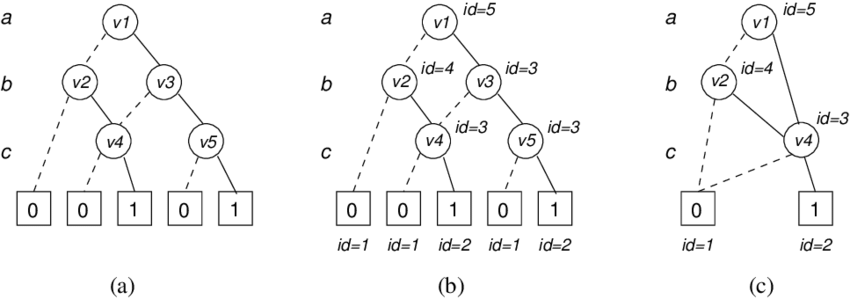
\includegraphics[width=0.8\linewidth]{figures/robdd-example.png}
    \caption{\cite{dhiraj-2023} Example of ROBDD construction for $f=(a \lor b) \land c$; a) OBDD for the variable order a,b,c; b) OBDD with unique identifiers; c) ROBDD for variable order a, b, c.}
    \label{fig:robdd-construction-example}
\end{figure}

From now on whenever it is written BDD, we mean ROBBD, because ROBDD are the only type of BDDs exploited in both practice and theory.
Since BDDs represent Boolean formulas, on them can be applied the common Boolean operations.
Given two BDDs $B_0$ and $B_1$ and denoting with $f(B_0)$ and $f(B_1)$ the two formulas represented by the two BDDs, the common Boolean operations that can be applied on them are:
\begin{itemize}
    \item $and(B_0,B_1)$, returning the ROBDD for the formula $f(B_0) \land f(B_1)$;
    \item $or(B_0,B_1)$, returning the ROBDD for the formula $f(B_0) \lor f(B_1)$;
    \item $not(B_0)$, returning the ROBDD for the formula $\neg f(B_0)$;
    \item $diff(B_0,B_1)$, returning the ROBDD for the formula $f(B_0) \land \neg f(B_1)$;
    \item $exists(B_0,X)$, returning the ROBDD for the formula $\exists X.f(B_0)$;
    \item $forall(B_0,X)$, returning the ROBDD for the formula $\forall X.f(B_0)$;
    \item $rename(B_0,X,Y)$, returning the ROBDD obtained by renaming variables in $X$ to $Y$;
    \item $restrict(B_0,X,1)$ and $restrict(B_0,X,0)$, returning the ROBDD for the formula $f(B_0)[1/X]$ and $f(B_0)[0/X]$, respectively the positive and negative co-factors.
\end{itemize} 

The complexity of each of the above operations is $O(\card{B_0})$ for unary ones and $O(\card{B_0} \cdot \card{B_1})$ for binary ones, with $\card{B}$ meaning the number of nodes of a given BDD $B$.

In order to apply BDDs to model checking, we need to interpret the whole state machine and sets of states as Boolean variables or Boolean formulas .

%!TEX root = ../../main.tex

\section{The AIGER format}

This section presents an important format highly used in model checking and reactive synthesis: AIGER. 

The AIGER format is used to describe circuits by multi-rooted And-Inverter Graphs (AIG) with latches that store the system state. It was developed as a compact and simple file format benchmarks for the hardware model checking competition (HWMCC). 
A And-Inverter Graph is a directed, acyclic graph that represents a structural implementation of the logical functionality of a circuit or network. An AIG consists of two-input nodes representing logical conjunction, terminal nodes labeled with variable names and edges optionally containing markers indicating logical negation. This representation of a logic function is rarely structurally efficient for large circuits, but is an efficient representation for the manipulation of Boolean functions.
Conversion from the network of logic gates to AIGs is fast and scalable. It only requires that every gate be expressed in terms of AND and NOT gates.
This conversion does not lead to unpredictable increase in memory use and runtime. This makes AIG an efficient representation in comparison with either the binary decision diagram (BDD) or the sum-of-product ($\Sigma o \Pi$) form.

% TODO: example of aig?

A file in AIGER format (ASCII variant) consists of the following parts: header, input definitions, latch definitions, output definitions and and-gate definitions. The header consists of a single line \lstinline{aag M I L O A}, where \lstinline{M} gives the maximum variable index, \lstinline{I} the number of inputs, \lstinline{L} the number of latches, \lstinline{O} the number of outputs and \lstinline{A} the number of AND gates.
Boolean variables are referred by even numbers, while odd numbers are referred to the negation of a variable, i.e. if $n$ is even, $n+1$ is the negation of $n$. $0$ and $1$ are special indexes referring the false and true values, respectively.
Then, the format can be divided in 5 sections declared in the header.

\begin{lstlisting}[caption=The empty circuit without inputs nor outputs and constant false/true in AIGER format]
aag 0 0 0 0 0             header

aag 0 0 0 1 0             header
    0                     output

aag 0 0 0 1 0             header
    1                     output
\end{lstlisting}

Every input definition takes one line and consists of a single even number.
Every latch definition takes one line and consists of an even number, followed by a number that defines which variable is used to update the latch in every step. The initial value is given by an additional number between either 0, 1 or the latch itself, which means to set the initial value to false, true or undefined, respectively. By default latches are assumed to have initial value 0.
Every output definition takes one line and consists of a single number, representing a possibly negated input, latch or and-gate. 
Every and-gate definition takes one line and consists of three numbers. The first is an even number, representing the output of the and-gate, and is followed by two numbers representing its (possibly negated) inputs.
There are also two further optional sections: symbol table and comments. The symbol table assigns names to inputs, latches and outputs. It is optional, and need not be complete. Every line defines the name of one input, latch, or output, and starts with i, l, o, respectively,
followed by the number of the input, latch, or output in the sequence of definitions.

As notable example we want to show how to encode a full-adder in AIGER format. A full-adder needs no presentation, it is just a circuits which sum two bits considering the carry.
Usually, a full-adder has three inputs: the two addends and the carry of the previous sum. That's because a full-adder is designed to be chained to other full-adders in order to sum sequence of bits. 
The first full-adder has carry value set to false, while the $i$ full-adder has the carry value in input set to the $i-1$ full-adder carry output. 
In our example, the full-adder is designed to be used as a stand-alone circuit where the carry result is saved in a latch and is used in the next computation, and it is $0$ initially.
Basically, this design choice was made just to show how to encode latches in AIGER format.

\begin{figure}[!htp]
    \centering
    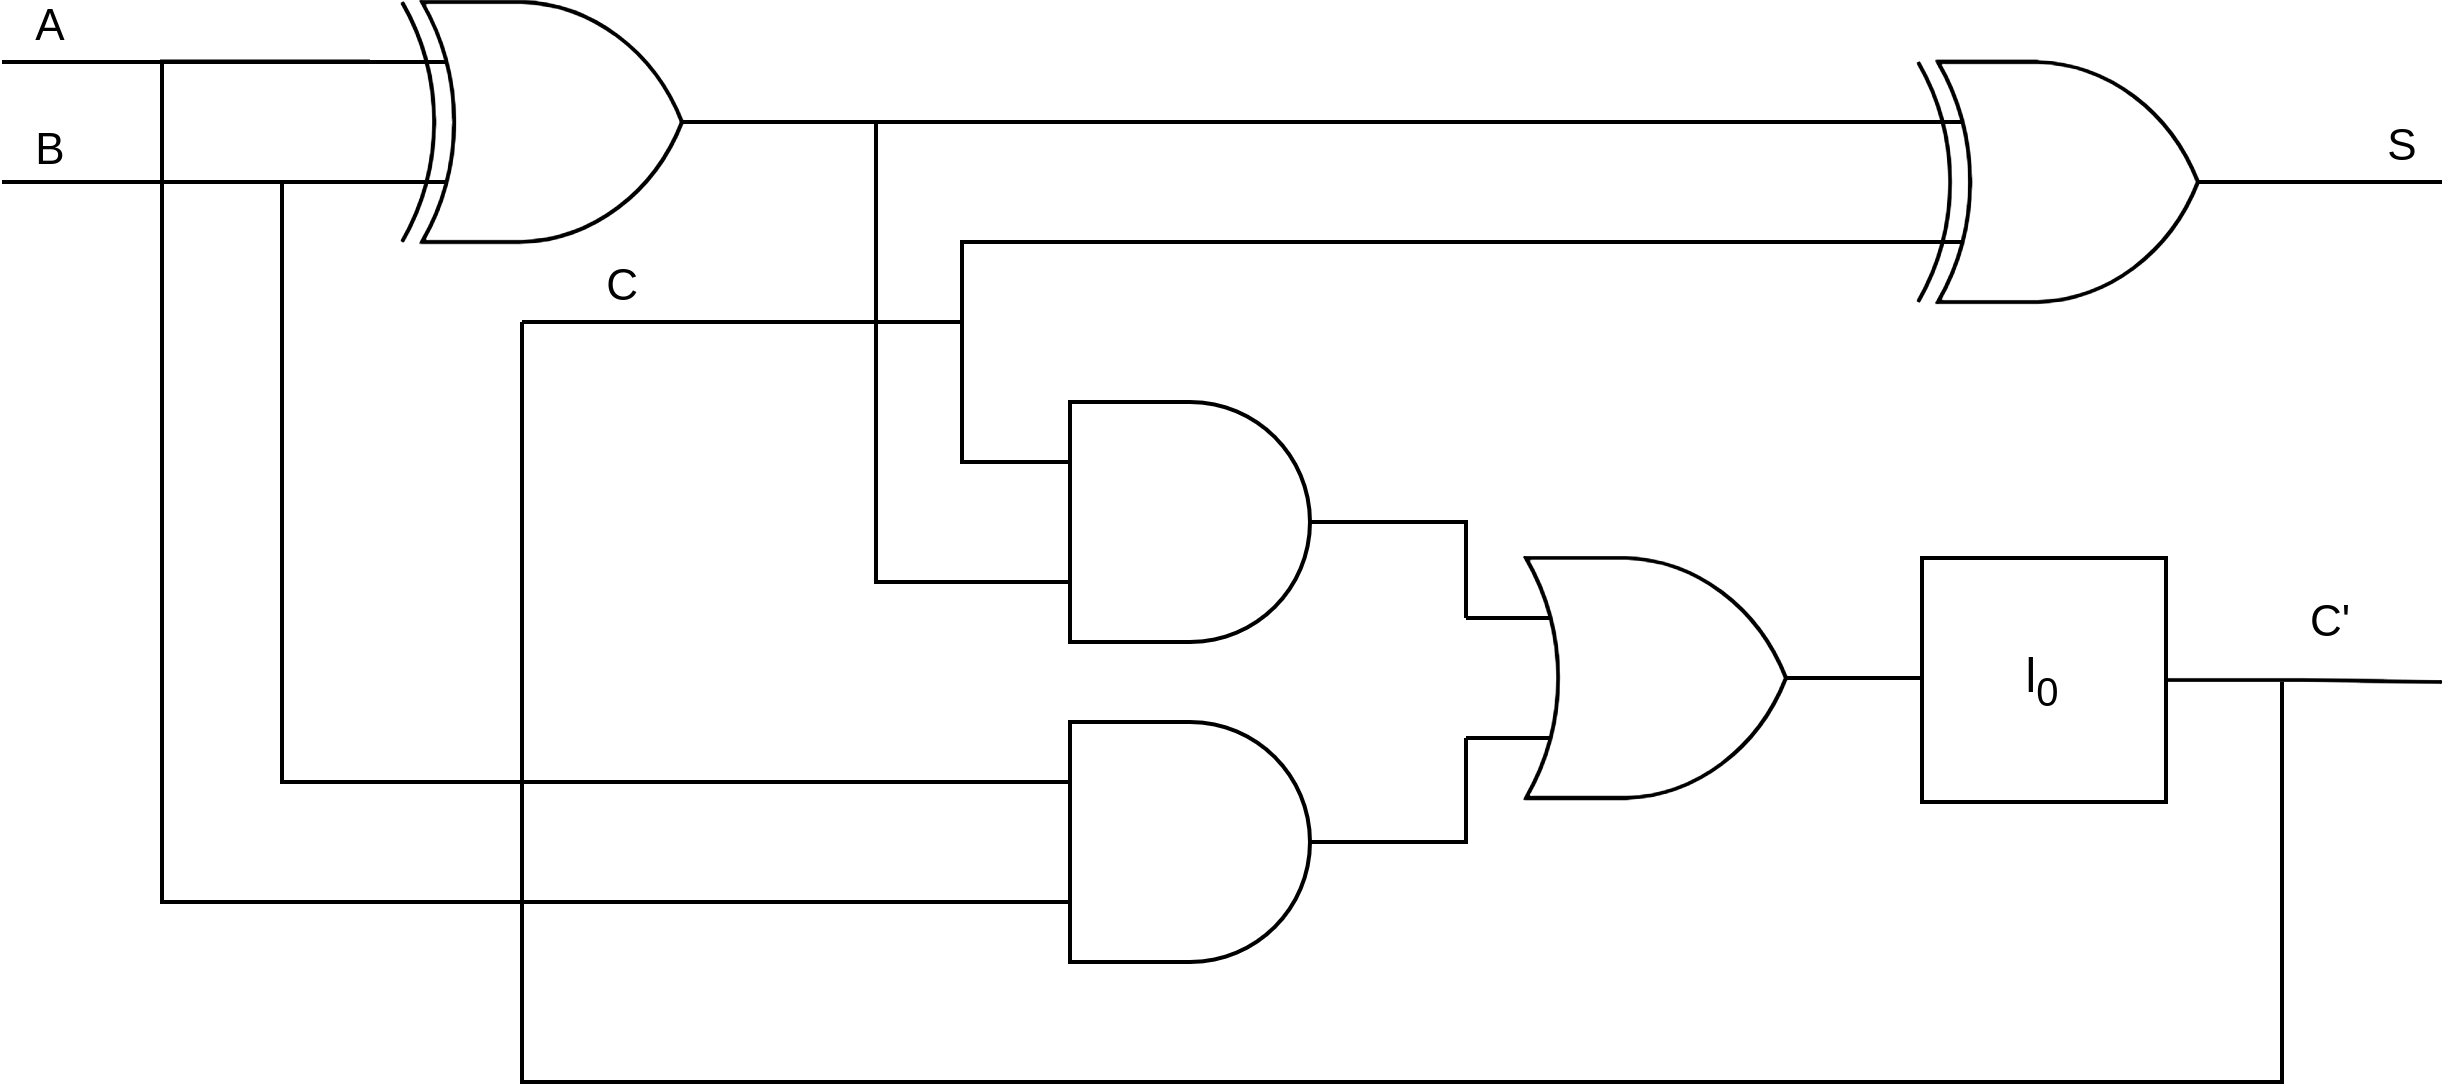
\includegraphics[width=0.6\linewidth]{figures/full-adder-circuit.png}
    \caption{Full adder circuit}
    \label{fig:full-adder-circuit}
\end{figure}

To encode a full-adder we have to express two formulas by just using and and not gates: the sum result and the carry result.
The sum result is given by $S = (A \oplus B) \oplus C$, while the carry result $C' = (A \land B) \lor (C \land (A \oplus B))$. $A$, $B$ are the input bits and $C$ the carry value.
The first step is to convert the formula to Conjunctive Normal Form (CNF) and then remove the or gates by De Morgan's laws. 

\begin{figure}
    \centering
\begin{flalign*}
& (A \oplus B) \oplus C \\
& \iff \text{(by CNF)} \\
& (\neg A \lor \neg B \lor C) \land (\neg A \lor B \lor \neg C) \land (A \lor \neg B \lor \neg C) \land (A \lor B \lor C) \\
& \iff \text{(by De morgan's laws)} \\
& \neg(A \land B \land \neg C) \land \neg(A \land \neg B \land C) \land \neg(\neg A \land B \land C) \land \neg(\neg A \land \neg B \land \neg C)
\end{flalign*}
    \caption{Expressing full-adder sum result via $\land$ and $\neg$ gates}
\end{figure}

\begin{figure}[!htp]
    \centering
    \begin{flalign*}
    & (A \land B) \lor (C \land (A \oplus B)) \\
    & \iff \text{(by CNF)} \\
    & (A \lor B) \land (A \lor C) \land (B \lor C) \\
    & \iff \text{(by De Morgan's laws)} \\
    & \neg(\neg A \land \neg B) \land \neg(\neg A \land \neg C) \land \neg(\neg B \land \neg C)
    \end{flalign*}
    \caption{Expressing full-adder carry result via $\land$ and $\neg$ gates}
\end{figure}

\begin{lstlisting}[caption = Full-adder in AIGER format]
agg 19 2 1 2 16
    2             input A
    4             input B
    6 14          latch C
    38            output sum
    16            output carry
    -- carry result
    8  3  5       !A & !B
    10 3  7       !A & !C
    12 5  7       !B & !C
    14 9  11      !(!A & !B) & !(!A & !C)
    16 14 13      !(!A & !B) & !(!A & !C) & !(!B & !C)
    -- sum result
    18 2  4       A & B
    20 18 7       A & B & !C
    22 2  5       A & !B
    24 22 6       A & !B & C
    26 3  4       !A & B
    28 26 6       !A & B  & C
    30 3  5       !A & !B 
    32 30 7       !A & !B & !C
    34 21 25      !(A & B & !C) & !(A & !B & C)
    36 34 29      !(A & B & !C) & !(A & !B & C) & !(!A & B & C)
    38 36 33      !(A & B & !C) & !(A & !B & C) & !(!A & B & C) & !(!A & !B & !C)
    i0 A
    i1 B
    o0 sum
    o1 carry
    Full adder in AIGER format
\end{lstlisting}

The usual AIGER format can not cope with reactive synthesis, so in \cite{jacobs2014extended} has been proposed an extended AIGER format for controller synthesis. They suggest to reserve the special string \lstinline{controllable_} and pretend it to the names of controllable input variables. 
All other input variables are implicitly controlled by the environment.

%!TEX root = ../../main.tex

\section{The SMV language}
\label{sec:smv}

The algorithms presented in this thesis have been implemented in the model checker nuXmv, a symbolic model checker for the analysis of synchronous finite-state and infinite-state systems \cite{CCD14}. It implements state-of-the-art algorithms for model checking, using SMV as modeling and specification language.

SMV is a language to describe finite state synchronous models. 
The code is divided in modules, which is a template for a state transition system and can be used to model multiple components in a system through multiple instances. 
Instances of modules can be used in the definitions of other modules, giving the possibility to define hierarchical models of complex systems.
Each model is a module, defined by the keyword \lstinline{MODULE} and a name followed by a list of the module input variables. State variables determine the state space of a model and they are defined in a list beginning with the keyword \lstinline{VAR}. 
The SMV language provides Booleans, enumerative, bounded integers and words (arrays of Booleans which allow bitwise logical and arithmetic operations) as data type and arrays.
Each state variable requires the definition of its initial state and next state (transitions), by the statements \lstinline{init(name) := expression} and \lstinline{next(name) := expression}.
The transitions and initial state may be non-deterministic.
Additional variables can be defined following the keyword \lstinline{DEFINE}.
The expressions are expressed by state variables, input variables and the next value of a variable with \lstinline{next(var)}. 
The allowed operators are: 
\begin{flalign}
& +,\; -,\; *,\; /,\; mod \tag{Arithmetical operators} \\ 
& <,\; \leq,\; >,\; \geq,\; =,\; \neq \tag{Comparison operators} \\
& \&,\; |,\; !,\; xor,\; \to,\; \iff \tag{Logical operators}
\end{flalign}

An interesting expression is the conditional expression, defined by
\begin{lstlisting}[language=smv, mathescape=true]
case 
    $guard_1$ : $expression_1$; $\dots$ $guard_n$ : $expression_n$; 
    TRUE: $expression_{n+1}$; 
esac
\end{lstlisting}
where $guard_1 \dots guard_n$ are guards sequentially evaluated. If a $guard_i$ is true, then the conditional expression is evaluated to $expression_i$, otherwise is evaluated to $expression_{n+1}$.

Instances of modules can be used to build other modules and are instantiated by variable definitions. A module can be instantiated more the once and one module in the SMV model must have the name \lstinline{main}. This is the top module in
the composition hierarchy. The specifications to be verified can be written in $CTL$, by the keyword \lstinline{CTLSPEC}, or $\ltl$, by the keyword \lstinline{LTLSPEC}, or invariant ones, by the keyword \lstinline{INVAR}. 
Invariant specifications are Boolean expressions that must hold forever.

An example showing what we explained previously is the ferryman puzzle.
Briefly, there is a ferryman who wants to cross a river with three things: a cabbage, a goat and a wolf. The difficulty lies on making everything cross the river under some constraints:
\begin{itemize}
    \item ferryman carries only one passenger i.e. ferryman plus another thing;
    \item goat will eat cabbage when left alone;
    \item wolf will eat goat.
\end{itemize}
We split the implementation in plant and controller modules.
The first module to be designed is the plant and, as already said in \autoref{sec:ltl-model-checking}, the plant model is meant to define the constraint of the system. 
In particular, we define how all four elements behave. 
There are four state vars each of which can assume value either \lstinline{right} or \lstinline{left}. 
There is only one input variable, i.e. \lstinline{move}, defining the move to perform on the plant. 
The move can be: \lstinline{c}, carry cabbage, \lstinline{g}, carry goat, \lstinline{w}, carry wolf, and \lstinline{e}, carry nothing.
Afterwards, we set the initial state of each state variable to \lstinline{right}, i.e. the right side of the river. 
The next transition of goat, wolf and cabbage is defined as a case expression: if the move is not to carry that element and the element has the same position as man, then nothing changes; otherwise, that is the move is to carry such element and the man has the same position, we change the position of such element, so if it is on the right, the next transition brings it to the left, and vice-versa.
In order to make the code more readable, we describe some defines: \lstinline{no_carry}, \lstinline{carry_goat}, \lstinline{carry_wolf}, \lstinline{carry_cabbage},  \lstinline{safe_state} defining the condition for a state to be a safe state, i.e. whenever the goat and the wolf or the goat and the cabbage are in the same position, the man has the same position as goat to keep someone from getting eaten, and \lstinline{goal}, i.e. all elements are at the left bank.

\begin{lstlisting}[language=smv, caption=Ferryman example: plant module]
MODULE plant(move)
  VAR
    man     : {right, left};
    wolf    : {right, left};
    goat    : {right, left};
    cabbage : {right, left};
  DEFINE
    no_carry      := move=e;
    carry_goat    := move=g;
    carry_wolf    := move=w;
    carry_caggabe := move=c;
    safe_state := goat = wolf | goat = cabbage -> goat = man;
    goal := cabbage = left & goat = left & wolf = left & man = left;
  ASSIGN
    init(man)     := right;
    init(goat)    := right;
    init(wolf)    := right;
    init(cabbage) := right;
  ASSIGN
    next(cabbage) := case
      !(carry_caggabe & cabbage=man) : cabbage;
      cabbage=right : left;
      cabbage=left  : right;
    esac;
    next(goat) := case
      !(carry_goat & goat=man) : goat;
      goat=right : left;
      goat=left  : right;
    esac;
    next(wolf) := case
      !(carry_wolf & wolf=man) : wolf;
      wolf=right : left;
      wolf=left  : right;
    esac;
    next(man) := case
      man=right : left;
      man=left  : right;
    esac;
\end{lstlisting}

The controller is meant to observe the plant state by input variables and chose the next move in order to reach the goal passing only through safe states.
\begin{lstlisting}[language=smv, caption=Ferryman example: controller module]
MODULE controller(cabbage,goat,wolf,man)
VAR
  move : {c, g, w, e};
ASSIGN
  move = case
      man=right: case
          man=cabbage & man=goat & man=wolf: g;
          man=cabbage & man=goat: c;
          man=cabbage & man=wolf: w;
          man=cabbage: c;
          man=goat & man=wolf: w;
          man=goat : g;
          man=wolf : w;
          TRUE : e;
        esac;
      TRUE: case
          man=cabbage & man=goat: c;
          man=goat & man=wolf: g;
          TRUE: e;
      esac;
    esac;
\end{lstlisting}

Last but not least, the main module set the closed-loop between plant and controller.
To check the correctness of the system we may check whether the $\ltl$ formula \lstinline{p.safe_state U p.goal}, that is until we do not reach the goal state, all visited states were safe. 

\begin{lstlisting}[language=smv, caption=Ferryman example: main module]
MODULE main
VAR
  p: plant(c.move);
  c: controller(p.cabbage,p.goat,p.wolf,p.man);
LTLSPEC
  p.safe_state U p.goal
\end{lstlisting}

%!TEX root = ../../main.tex

\section{Reactive Synthesis}
\label{sec:reactive-synthesis}

Finally, we have reached the main topic of my thesis: Reactive Synthesis.

Reactive synthesis is the problem of translating a logical specification into a reactive system that is guaranteed to satisfy the specification for all possible behaviors of its environment. 
It differs from LTL Model Checking by the fact that we are not interested in figure out whether a given property $\phi$ holds in a model $\model$, but we want to generate a model $\model'$ automatically such that $\model' \models \phi$ by construction. 
In this case we say that the synthesized model $\model'$ is correct by construction.
Such model is a reactive system because its output is determined by reacting to the input values and formulated as either a Mealy Machine or a Moore Machine. 
The problem was introduced by Alonzo Church more than $60$ years ago \cite{C64}. 
Recent years have brought advances both in reasoning methods that can be used as tools in the synthesis process and in the synthesis approaches themselves.
As a result, the complexity of the synthesized systems has risen steadily. 
However, the logical and algorithmic foundations of the synthesis problem are still far from complete.

All algorithms to solve the Reactive Synthesis problem are based on game theory, in particular we can look at such problem like a two-players infinite games on finite graphs (\cite{R68}, \cite{W95}, \cite{BL90}). 
The main player is called Controller, or $P_0$, while the other player is called Environment, or $P_1$. 
Each player has a set of variables that can control and, since the game is seen from the perspective of $P_0$, the variables controlled by $P_0$ are called controllable and the ones controlled by $P_1$ are called uncontrollable.
In this type of games, it is chosen a-priori who performs the first move. 
It could be that $P_0$ moves first, it could be that $P_1$ moves first, or it could be that $P_0$ and $P_1$ move simultaneously. 
Along all the thesis we assume that $P_1$, the Environment, moves first and that every synthesized model is a Mealy Machine.

Let us start defining the Reactive Synthesis problem formally. 
In the following definition there are a lot of terms that could be unknown at first glace, but no worries because they are explained in the next sub-sections.

\begin{definition}[\cite{jacobs2015} Reactive Synthesis problem]
Let $\phi$ be a temporal formula over the alphabet $\Sigma = \C \cup \U$. We say that $\phi$ is realizable if and only if there exists a strategy $g \colon (2^\U)^+ \to 2^\C$ such that $U = \tuple{U_0,U_1,\dots} \in (2^\U)^\omega$, it holds that $g(U) \models \phi$. 
The synthesis problem is the decision problem to say whether $\phi$ is realizable or not. If $\phi$ is realizable, the corresponding strategy $g$ is computed.
\end{definition}

\subsection{Infinite game on graphs}
As we have already said previously, the reactive synthesis problem is reduced to infinite games on graphs.
There are some basic concepts which must be fixed before moving forward, in particular: the concept of an arena, what a strategy is, the concept of game and what we mean with winning region.

An \textit{arena} is the battlefield where two players clash. It is a finite graph, therefore it has some vertices and edges, and each player controls a subset of vertices. Controlling a vertex means to be able to select the edge and so the next vertex.   
Note that there are no vertices controlled by both players at the same time.
Whenever the two players play, they define the so called \textit{play} of the arena, which consists in the sequence of vertices crossed during the game. 
During the game both players do not act with out any logic, but they follow a \textit{strategy}. Such strategy is basically a function reading the play made so far, i.e. the sequence of vertices crossed so far, and select the next vertex to go. 
A strategy is called \textit{positional}, or memoryless, if the next vertex is chosen according to the current vertex and no the previous ones. 

\begin{definition}[\cite{infinite-games} Arena]
An arena $\arena = (V, V_0, V_1, E)$ consists of:
\begin{itemize}
    \item a finite set $V$ of vertices;
    \item disjoint subsets $V_0,V_1 \subseteq V = V_0 \cup V_1$ denoting the vertices of Player 0 and Player 1 respectively, and
    \item a set $E \subseteq V \times V$ of directed edges such that every vertex has at least one outgoing edge, i.e. $\set{v' \; | \; (v,v') \in E}$ is non-empty for every $v \in V$.
\end{itemize}
\end{definition}

\begin{definition}[\cite{infinite-games} Play]
A play in an arena $\arena = \tuple{V, V_0, V_1, E}$ is an infinite sequence $\rho=\rho_0\rho_1\rho_2\dots \in V^\omega$ such that $(\rho_n,\rho_{n+1}) \in E$ holds for every $n \in \Nat$. 
The set of plays in $\arena$ is denoted by $Plays(\arena)$, the set of all plays starting in $v$ by $Plays(A,v)$, and we define $Plays(A,V')=\bigcup_{v\in V'} Plays(\arena,v), \; \forall V' \subseteq V$.
\end{definition}

\begin{definition}[\cite{infinite-games} Strategy]
A strategy for Player $i \in \{0,1\}$ in an arena $\arena = \tuple{V,V_0,V_1,E}$ is a function $\sigma \colon V^*V_i \to V$ such that $\sigma(wv)=v' \implies (v,v') \in E,\; \forall w \in V^*,\; \forall v \in V$. 
\end{definition}

\begin{definition}[\cite{infinite-games} Consistent Play]
A play $\rho = \rho_0\rho_1\rho_2\dots$ in an arena $\arena=\tuple{V,V_0,V_1,E}$ is consistent with a strategy $\sigma$ for Player $i$ in $\arena$ if, $\rho_{n+1} = \sigma(\rho_0\dots\rho_n)$ for every $n \in \Nat$ with $\rho_n \in V_i$. 
Given a vertex $v$, we denote the set of plays that are consistent with $\sigma$ and start in $v$ with $Plays(\arena, v, \sigma)$. 
Finally, we define $Plays(\arena, V', \sigma)$ for $V'\subseteq V$ by $Plays(\arena, V', \sigma) = \bigcup_{v \in V'} Plays(\arena, v, \sigma)$.
\end{definition}

\begin{definition}[\cite{infinite-games} Positional (Memoryless) Strategy]
A strategy $\sigma$ for Player $i$ in an arena $\arena=(V,V_0,V_1,E)$ is positional (or memoryless) if $\sigma(wv)=\sigma(v)$ for all $w \in V^*$ and $v \in V$. 
Equivalently, a positional strategy can be seen as a function $\sigma \colon V_i \to V$.
\end{definition}

Only the arena is not enough to play a \textit{game}, but we need a winning condition.
When we set the winning condition, we call \textit{winning strategies} all those strategies which allow to win. 
The concept of winning strategies is connected to the one of \textit{winning region}, that is the set of all vertices starting from which a player has a winning strategy.
Therefore, we can reduce the reactive synthesis problem to find such winning region and, if it exists, then extract a strategy from it.

\begin{definition}[\cite{infinite-games} Game]
A game $\game=\tuple{\arena,Win}$ consists of an arena $\arena$ with vertex set $V$ and a set of winning sequences $Win \subseteq V^\omega$. 
We call a sequence $\rho$ winning for Player $0$ if and only if $\rho \in Win$ and winning for Player $1$ otherwise.
\end{definition}

\begin{definition}[\cite{infinite-games} Winning strategy]
Let $\game=(\arena,Win)$ be a game. A strategy $\sigma$ for Player $i$ in $\arena$ is a winning strategy from a vertex $v \in V$ if every play that is consistent with $\sigma$ and starts in $v$ is winning for Player $i$, i.e. if $Plays(\arena, v, \sigma) \subseteq Win$ for $i=0$ and $Plays(\arena, v, \sigma) \subseteq V^\omega \setminus Win$ for $i=1$. 
\end{definition}

\begin{definition}[\cite{infinite-games} Winning region]
The winning region $W_i(\game)$ of Player $i$ in a game $\game$ is the set of vertices from which Player $i$ has a winning strategy.
\end{definition}

\begin{definition}[\cite{infinite-games} Determinancy and Positional Determinancy]
Let $\game$ be a game with vertex set $V$. We say that $\game$ is determined if $W_0(\game)\cup W_1(\game) = V$. Furthermore, we say that $\game$ is positionally determined if, from every vertex $v \in V$ one of the players has a positional winning strategy.
\end{definition}

\begin{definition}[\cite{infinite-games} Uniform Positional Winning Strategy]
Let the game $\game=(\arena, Win)$. A strategy $\sigma$ for Player $i$ is a uniform positional winning strategy if it's positional and winning from every vertex in $W_i(G)$.
\end{definition}

\begin{figure}
    \centering
    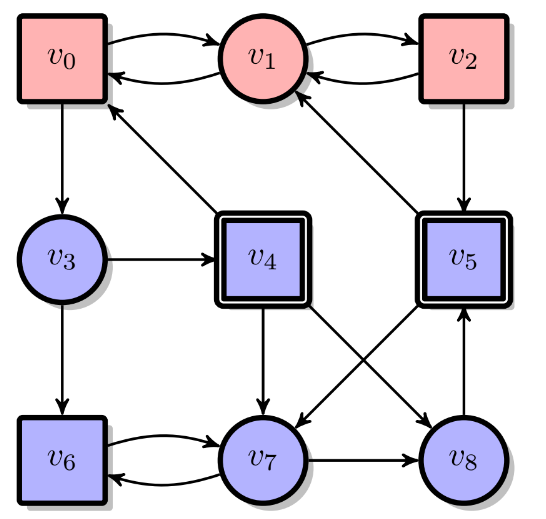
\includegraphics[width=0.4\linewidth]{figures/arena-example.png}
    \caption{\cite{infinite-games} Example of arena. The winning condition of player $0$ is to reach doubly-lined framed vertices (reachability game). Circular vertices are controlled by $P_0$, while rectangular ones are controlled by $P_1$. Blue and red vertices are $P_0$ and $P_1$ winning regions, respectively}
    \label{fig:enter-label}
\end{figure}

% \begin{lemma}
% For any game $\game$, it holds that $W_0(\game) \cap W_1(\game) = \emptyset$. In other words, the winning region of a player $i$ is the complement of the winning region for the player $1-i$, i.e. $W_i(\game) = V \setminus W_{1-i}(\game)$.
% \end{lemma}


\subsection{Safety and Reachability games}
The easiest games to solve, but at the same time enough interesting to analyze, are safety and reachability games.
Safety games consists in a game on an arena where we want to stay forever in a subset of vertices of the arena. In this case $P_0$ tries to stay forever in such subset, while $P_1$ tries to reach an outer vertex.
Reachability games consists in a game on an arena where we want to reach a subset of vertices of the arena. In this case $P_0$ tries to reach such subset, while $P_1$ tries to prevent $P_0$ to reach it by staying forever in the complement subset of vertices.

As maybe you could notice, safety and reachability games are dual: when $P_0$ is playing a safety game, $P_1$ is playing a reachability game, while when $P_0$ is playing a reachability game, $P_1$ is playing a safety game.

\begin{definition}[\cite{infinite-games} Occurrence set]
Given a play $\rho$, we denote as $Occ(\rho)$ the set of vertices occurring in $\rho$.
\end{definition}

\begin{definition}[\cite{infinite-games} Reachability game]
Let $\arena=\tuple{V, V_0, V_1, E}$ be an arena and let $R \subseteq V$ be a subset of $\arena$'s vertices. Then, the reachability condition $Reach(R)$ is defined as
\begin{flalign*}
    Reach(R) = \set{\rho \in V^\omega \; |\; Occ(\rho) \cap R \neq \emptyset}
\end{flalign*}
We call a game $\game = (\arena, Reach(R))$ a reachability game with reachability set $R$.
\end{definition}

\begin{definition}[\cite{infinite-games} Safety game]
Let $\arena = \tuple{V, V_0, V_1, E}$ be an arena and let $S \subseteq V$ be a subset of $\arena$'s vertices. Then, the safety condition $Safety(S)$ is defined as 
\begin{flalign*}
    Safety(S) = \set{\rho \in V^\omega \; | \; Occ(\rho) \subseteq S}
\end{flalign*}
We call a game $\game = (\arena, Safety(S))$ a safety game with safety set $S$.
\end{definition}

\begin{definition}[\cite{infinite-games} Dual Arena]
Let $\arena = \tuple{V,V_0,V_1,E}$ be an arena. The dual arena $\bar{\arena}$ of $\arena$ is defined as $\bar{\arena} = \tuple{V,V_1,V_0,E}$. 
\end{definition}

\begin{theorem}[\cite{infinite-games} Duality between safety and reachability games]
Let $\arena = \tuple{V,V_0,V_1,E}$ be an arena, let $\game = \tuple{A, SAFETY(S)}$ be a safety game with $S \subseteq V$ and define the reachability game $\game' = \tuple{\bar{\arena}, REACH(V \setminus S)}$. Then $W_i(\game) = W_{1-i}(\game')$ for each $i \in \set{0,1}$.
\end{theorem}

Let us now speak about algorithms to solve safety and reachability games. 
First of all, permit us to introduce some basic algorithms for solving such games on an explicit representation of the arena.
Afterwards, we will see that such algorithms can be empowered by BDD solving the games expressing the arena symbolically,

The fundamental algorithm to solve reachability is an algorithm based on fix-point computation of the 0-attractor. 
Basically, fixed a subset $R \subseteq V$ that we want to reach, we start computing the set of vertices from which the player $P_0$ can force to visit $R$ and $P_1$ can not avoid to visit $R$. Given such set of vertices we union with $R$ and do the same computation but now instead of reaching just $R$, we want to reach the new set resulting from the previous union. Going on like that we reach a point where the new computed set is not increasing anymore. 
That is the so-called fixed-point. 
We are sure to reach it because the set of vertices is finite.

\begin{definition}[\cite{infinite-games} i-Attractor]
Let $\game = (\arena, Reach(R))$ be a reachability game, where $\arena = \tuple{V, V_0, V_1, E}$ and $R \subseteq V$, and let $i \in \set{0,1}$ determine a player.
The controlled predecessor $CPre_i(R)$ of $R$ is defined as
\begin{flalign*}
CPre_i(R) = & \set{v \in V_i \; | \; \text{$v' \in R$ for some successor $v'$ of $v$}}\;\cup \\
            & \set{v \in V_{1-i} \; | \; \text{$v' \in R$ for all successors $v'$ of $v$}}
\end{flalign*}
The i-Attractor $Attr_i(R)$ in $\arena$ is defined by inductively applying the controlled predecessor via
\begin{flalign*}
& Attr_i^0(R) = R \\
& Attr_i^{n+1}(R) = Attr_i^n(R) \cup CPre_i(Attr_i^n(R)) \\
& Attr_i(R) = \bigcup_{n \in \Nat} Attr_i^n(R).
\end{flalign*}
Note that $Attractor_i^n \subseteq Attractor_i^{n+1}$ for all $n \geq 0$
\end{definition}

After having reached a fixed-point, we end up with a set of vertices which coincides with the winning region of $P_0$. 
Extracting a strategy from every nodes is easy. 
First save all controlled predecessors $CPre_0^0,\dots,CPre_0^n$, with $n \in \Nat$ such that $Attr_i^{n+1}(R) = Attr_i^{n}$ (we reached a fixed-point at attractor $n$) and $CPre_0^0 = R$. Then, we start from the last controlled predecessor $CPre_0^n$ and for each vertex $v \in CPre_0^n$ and $ v \in V_0$, we select an edge $\tuple{v,v'} \in E$ such that $v' \in CPre_0^{n-1}$. 
In other words, $P_0$ visits only those vertices from which $P_1$ can not avoid to get closer to the subset $R$, ending up in $CPre_0^9$ which is exactly the subset $R$. 
The strategy computation can be integrated in the algorithm in order to be more efficient.

Now that we are able to solve reachability game, we are able to solve safety game as well by exploiting duality. 
Indeed, as we have already seen, solving a safety game $\game = \tuple{\arena, SAFETY(S)}$ for $P_0$ is the same as solving a reachability game in the dual game $\bar{\game} = \tuple{\arena, REACH(V \setminus S)}$. 
Therefore, by applying the 1-attractor computation on $\game$, we can easily compute the winning region $W_0(\game)$ for $P_0$ by taking the complement of the winning region for $W_1(\game)$, that is $W_0(\game) = V \setminus W_1(\game)$.
Extracting a strategy for a safety game is easier.
Given a winning region $W_0(\game)$, for each vertex $v \in W_0(\game)$ and $v \in V_0$, we select an edge $\tuple{v,v'} \in E$ such that $v' \in W_0(\game)$. In other words, $P_0$ must visit only those vertices from which can be forced to stay in the winning region and so not escaping from $S$.

This algorithm based on fixed-point is very simple but also powerful because it allows to solve a reachability game, and therefore also safety games, in linear time. 

\begin{lemma}[\cite{infinite-games}]
Let $\game = (\arena, Reach(R))$ be a reachability game, where $\arena = \tuple{V, V_0, V_1, E}$ and $R \subseteq V$. Then, $W_0(\game) = Attr_0(R)$ and $W_1(\game) = V \setminus Attr_0(R)$.
\end{lemma}

\begin{lemma}[\cite{infinite-games}]
The attractor $Attr_i(R)$ in an arena $\arena$ with edges $E$ can be computed in linear time in $\card{E}$.
\end{lemma}


\subsection{Other types of games}
Besides safety and reachability games, there are many other types of games. 
In fact, safety and reachability games are the basis and are useful to synthesize safety formulas and co-safety formulas, respectively. 
Formulating more complex winning condition, we end up with different games useful for many reasons explored later.

% As we have already seen, there exist formulas which do not belong to neither of the two fragments. Such formulas require more sophisticated games, each of which is a generalization of some other games.  
So far we have studied games there the winner is determined by a prefix, but there are games where no prefix determines the winner: B{\"u}chi and co-B{\"u}chi games.
The winning condition for B{\"u}chi games is that some states in a set of states are visited infinitely many times.
The winning condition for co-B{\"u}chi games is that exactly all states visited infinitely many times are subset of a given set of states.

\begin{definition}[\cite{infinite-games} States visited infinitely many times]
Given a play $\rho$, we denote as $Inf(\rho)$ all states visited infinitely many times during the play.
\end{definition}

\begin{definition}[\cite{infinite-games} B{\"u}chi games]
Let $\arena = \tuple{V,V_0,V_1,E}$ be an arena and let $F \subseteq V$ be a subset of vertices. Then, the B{\"u}chi condition B{\"u}chi(F) is defined as
\begin{flalign*}
    \text{B{\"u}chi(F)} = \set{\rho \in V^\omega \; | \; Inf(\rho) \cap F \neq \emptyset}
\end{flalign*}
We call a game $\game = \tuple{\arena, \text{B{\"u}chi(F)}}$ a B{\"u}chi game.
\end{definition}

\begin{definition}[\cite{infinite-games} Co-B{\"u}chi games]
Let $\arena = \tuple{V,V_0,V_1,E}$ be an arena and let $F \subseteq V$ be a subset of vertices. Then, the co-B{\"u}chi condition coB{\"u}chi(F) is defined as
\begin{flalign*}
    \text{coB{\"u}chi(F)} = \set{\rho \in V^\omega \; | \; Inf(\rho) \subseteq F}
\end{flalign*}
We call a game $\game = \tuple{\arena, \text{coB{\"u}chi(F)}}$ a co-B{\"u}chi game.
\end{definition}

A generalization of the are previous games are \textit{Parity games}. 
In parity games the vertices of the arena are colored by natural number and the goal of player $0$ is to ensure that the minimal color seen infinitely often on a play is even. 
Equivalently, player $i$ wins if and only if the minimal color seen infinitely often has parity $i$. 
Thus, the color of a vertex denotes its importance (smaller colors are more important than larger ones) and its value for the players (vertices of even color are desirable for $P_0$, but undesirable for $P_1$ and vice-versa). 
B{\"u}chi and co-B{\"u}chi games can be expressed as parity games with two colors.

\begin{definition}[\cite{infinite-games} Parity games]
Let $\arena = \tuple{V,V_0,V_1,E}$ be an arena and let $\Omega \colon V \to \Nat$ be a coloring function of vertices. Then, the parity condition $Parity(\Omega)$ is defined as
\begin{flalign*}
    Parity(\Omega) = \set{\rho \in V^\omega \; | \; \max \set{Inf(\Omega(\rho_0)\Omega(\rho_1)\Omega(\rho_2)\dots)}\text{ is even}}
\end{flalign*}
We call a game $\game = \tuple{\arena, Parity(\Omega)}$ a parity game.
\end{definition}

All above games are determined with uniform positional winning strategies.

\subsection{Solving Safety and Reachability games symbolically}
In real applications is impossible to synthesize models from a $\ltl$ formula exploiting explicit representation of the arena. 
That is because the number of states of the arena is exponential in the number of state variables, ending up with too large games.
A solution to this problem is exploiting symbolic representations of regions states which can be much smaller than the represented state space. 
After a brief introduction to reactive synthesis through its game theory formulation, let us adapt the previous algorithms to work on symbolic representations.

In the first place, we need to represent the arena symbolically. 
That can be done by interpreting as Boolean variables the state variables and Boolean formulas the transition relation. 
We do not need two different types of arenas, because a safety arena is suitable both safety and reachability games according to what $P_0$ wants to solve. 
Therefore, for simplicity we define only arenas for safety games. 
Afterwards, we need to adapt the i-attractor computation. 
The only aspect we need to change is the controlled predecessor computation, which now is expressed in terms of $\exists$. $\forall$, $\land$, $\lor$ and Boolean formulas. 
Thanks to BDDs all previous operations are much easier to perform, enchanting the equivalence check of formulas and keeping a compact representation during these computations.

\begin{definition}[\cite{jacobs2015} Symbolic representation of games]
A symbolic representation for a safety game is given as tuple $\arena = \tuple{L,X_u,X_c,T(L,X_u,X_c,L'),Unsafe(L)}$ where: (i) $L$ is a set of Boolean state variables; (ii) $X_u$ is a set of Boolean uncontrollable inputs; (iii) $X_c$ is a set of Boolean controllable outputs; (iv) $T(L,X_u,X_c,L')$ is the transition relation, given as a quantifier-free Boolean formula over variables $L$, $X_u$, $X_c$ and $L'$, which represents the values of the state variables after the transition; (v) $Unsafe(L)$ is the region of unsafe states.
\end{definition}

Unlike before, we define $0$-attractor and $1$-attractor separately just because we explain the different order of quantification. 
We recall that Environment player plays first, so all arguments are made under this important assumption.

For safety games there are two algorithms that we may exploit to solve them. 
The first algorithm is defined as in the previous sub-section, that is computing the $1$-attractor and then obtaining the winning region for $P_0$ by taking the complement the attractor. 
In this case we state the controlled predecessor of a set of states $Unsafe(L)$ as the set of states $CPre_1^i(Unsafe(L))$ such that there exists a valuation of the uncontrollable inputs for which for all valuations of the controllable inputs, there exists a transition to some states in $CPre_1^{i-1}(Unsafe(L))$.
The second algorithm exploits the analogy with $\mu$-calculus model checking.
Indeed, since the computation of the winning region for both safety and reachability games laid on fix-point computation, we can see the winning region for  reachability game as the result of the Least Fixed Point (LFP) computation, and the winning region for a safety game as the result of the Greatest Fixed Point (GFP) computation.

For reachability games, the computation of $0$-attractor is a little different from the $1$-attractor one. Since the Environment player starts playing, the controlled predecessor of a set of states $Unsafe(L)$ is stated as the set of states $CPre_0^i(Unsafe(L))$ such that for each valuation of the uncontrollable inputs for which there exists a valuation of the controllable input, there exists a transition to some states in $CPre_0^{i-1}(Unsafe(L))$.

\begin{definition}[\cite{jacobs2015} Symbolic controlled predecessor for safety games]
Given arena $\arena$ and a set of states $S \subseteq L$, the controlled predecessor for $P_1$ (1-attractor) of $S$ is defined as
\begin{flalign*}
CPre_1(A) = \exists X_u \forall X_c \exists L'. A(L') \land T(L,X_u,X_c,L')
\end{flalign*}
\end{definition}

\begin{definition}[\cite{jacobs2015} Symbolic controlled predecessor for reachability games]
Given arena $\arena$ and a set of states $S \subseteq L$, the controlled predecessor for $P_0$ (0-attractor) of $S$ is defined as
\begin{flalign*}
CPre_0(A) = \forall X_u \exists X_c \exists L'. A(L') \land Trans(L,X_u,X_c,L')
\end{flalign*}
\end{definition}

Another key point of reactive synthesis is the strategy extraction from the winning region.
Symbolically, a strategy is a relation among Boolean formulas defining states, uncontrollable variables and controllable variables. 
For safety games, given a state in the winning region and an uncontrollable variable, we relate them with all possible controllable variables values such that in any case the next transition is still in the winning region. 
For reachability games, we look for a strategy which allows us to get us closer and closer to the unsafe states until we reach them. We provide a formal definition of non-deterministic strategy for reachability game in \autoref{sec:non-deterministic-strategy-reachability-game}, since we have found no information about it on other papers.
Whenever we have a non-determinstic strategy, no matter if it is generated from safety game or a reachability one, we want to determinize it in order to encode it in a circuit.
In principle, any determinization of the strategy can be chosen to obtain a function strategy for the system player, but there are many optimizations applicable to reduce the size of it. 
The one we have chosen is called co-factor method with care-set optimization.
Starting with the $\lambda$ non-deterministic strategy represented symbolically we apply the following steps for each $x_c \in X_c$ controllable variable:
\begin{enumerate}
    \item we restrict $\lambda$ to one output $x_c$, denote as $\lambda_{x_c}$;
    \item we compute positive ($p$) and negative (n) co-factors of $\lambda_{x_c}$, i.e. the values $s$ and $x_u$ for which $\lambda_{x_c}(s,x_u)$ can be $1$ or $0$, respectively;
    \item the combinatorial inputs that are neither in the positive nor in the negative co-factor are outsize of the winning region, representing situations that cannot occur. Thus, $\lambda(s,x_u)$ must be true in $p \land \neg n$ and false in $\neg p \land n$, which give us the set of care states, named care-set;
    \item we minimize the positive co-factor with the care-set to obtain the value of function $\lambda(s,x_u)$;
    \item we substitute variable $x_c$ in $\lambda$ by $\lambda(s,x_u)$ since other controllable outputs may be related to it;
    \item finally, we proceed with the next variable.
\end{enumerate}
% Regarding reachability games, we define the non-deterministic winning strategy $\lambda$ of a game $\game$ as the union of smaller strategies $\lambda_1,\dots,\lambda_n$ each of which consists in a strategy to go from a controlled predecessor to next one.
% Since we have not found any algorithm implementing such procedure exploiting BDDs, we have formulated one presented in \autoref{chapt:original-contributions}.

\begin{definition}[\cite{jacobs2015} Strategy for safety games]
Let $\game$ be a safety game represented symbolically and $W_0(\game)$ be the winning region of $P_0$ for the safety game. 
A non-deterministic winning strategy $\lambda \subseteq \Bool^L \times \Bool^{X_u} \times \Bool^{X_c}$ is defined as:
\begin{flalign*}
    \lambda(s,x_u) = \set{x_c \in \Bool^L \; | \; s \in W(L) \land \forall L' . T(s,x_u,x_c,L') \to W(L')}
\end{flalign*}
Analogously, $\lambda$ can be described as follows talking about set of states, set of uncontrollable variables and set of controllable variables:
\begin{flalign*}
    \lambda(L,X_u,X_c) = \exists L'. W_0(L) \land T(L,X_u,X_c,L') \land W_0(L')
\end{flalign*}
\end{definition}

% \begin{definition}[Strategy for reachability games]
% Let $\game$ be a reachability game on a safety arena represented symbolically and $CPre_0^0,\dots CPre_0^n$ be the set of controlled predecessors of $P_0$ computed solving reachability game. Recall that $CPre_0^0 = Unsafe(L)$.
% We define a set of non-deterministic winning strategies $\lambda_1,\dots,\lambda_n$ such that $\lambda_i \subseteq \Bool^L \times \Bool^{X_u} \times \Bool^{X_c}$ for each $i \in [1,n]$ and is defined as:
% \begin{flalign*}
%     \lambda_i(s,x_u) = \set{x_c \in \Bool^L \; | \; s \in Cpre_0^i \land \forall L' . (T(s,x_u,x_c,L')) \to CPre_0^{i-1}(L')}
% \end{flalign*}
% The whole non-deterministic winning strategy $\lambda \subseteq \Bool^L \times \Bool^{X_u} \times \Bool^{X_c}$ is defined as
% \begin{flalign*}
%     \lambda = \bigcup_{i=1}^n \lambda_i 
% \end{flalign*}
% \end{definition}

\begin{algorithm}[!htp]
\caption{\cite{BLOEM20073} Algorithm to determinize any non-deterministic strategy}
\label{alg:functional-strategy}
\begin{algorithmic}[1]
\Procedure{ExtractFunctionalStrategy}{$\arena$, $\lambda$}
    \State initialize $f$ as a map from controllable variable to strategy
    \For{$x_c \in X_c$}
        \State $\lambda_{x_c} \gets \exists X_c \setminus \set{x_c}.\; \lambda$
        \State $p \gets \lambda_{x_c}[1/x_c]$
        \State $n \gets \lambda_{x_c}[0/x_c]$
        \State $\text{\textit{care-set}} \gets (p \land \neg n) \lor (\neg p \land n)$
        \State $f[x_c] \gets \text{$p$ minimized w.r.t. \textit{care-set}}$
        \State $\lambda \gets \lambda[f[x_c]/x_c]$
    \EndFor
    \Return $f$
\EndProcedure
\end{algorithmic}
\end{algorithm}

\subsection{Linear Temporal Logic synthesis}
In previous sub-sections we introduced the game-theory notions needed to deal with Reactive Synthesis. Now we can see how to exploit those games to synthesis correct-by-construction models starting from a $\ltl$ formula. 
We will not go into details since the aim of the thesis is to deepen safety and co-safety fragments of $\ltl$, but it is still important to be aware about the relation between and games and $\ltl$ classes of formulas. 
Each game allows to synthesize a specific class of $\ltl$ formulas following the temporal hierarchy (\ref{fig:temporal-hierarchy}): safety and co-safety by safety and reachability games, obligation by weak-parity games, recurrence and persistence by reachability B{\"u}chi and co-B{\"u}chi games and reactivity by parity games.

We can formalize the synthesis of a generic $\ltl$ formula $\phi$ as a game. 
Such game is played on an arena $\arena$ labelled by a function $l$, such that each vertex of $\arena$ is associated to a set of atomic propositions. 
The winning condition is that the formula $\phi$ is satisfied on all labelled plays induced by a strategy.

\begin{definition}[LTL game]
Let $\arena=\tuple{V,V_0,V_1,E}$ be an arena, $\mathcal{P}$ be a set of propositions and $l \colon V \to 2^\mathcal{P}$ be labeling of vertices by atomic propositions. Then, the $\ltl$ condition $LTL(\phi,l)$ is defined as
\begin{flalign*}
    LTL(\phi,l) = \set{\rho \in V^\omega \; | \; (l(\rho_0)l(\rho_1)l(\rho_2)\dots,0) \models \phi}
\end{flalign*}
We call a game $\game=\tuple{\arena,LTL(\phi,l)}$ a LTL game. 
\end{definition}

Every LTL game can be solved by reducing it to parity game. 
First we obtain the corresponding NBA to $\phi$. 
Then, we construct the arena by converting the NBA to Deterministic Parity Automaton and finally we solve it. 
The overall procedure is $2EXPTIME$-complete.

Nevertheless, we investigate only safety and co-safety fragments and so we can study only safety and reachability games. 
In $\autoref{sec:ebr-ltl-synthesis}$ is presented a procedure to build safety arenas starting from $\ebrltl$ formulas.

\subsection{AIGER format in Reactive Synthesis}
AIGER format is highly used in reactive synthesis field. Indeed, it is common to represent safety arenas and synthesized controllers in extended AIGER format for reactive synthesis.
In safety Arenans each latch represents a state, both controllable and uncontrollable variables are inputs and the only output is the value of the synthesized formula.
The initial state of games is the conjunction of all latches, according to their initial value, i.e. if a latch $l_0$ initial value if false, then the conjunction is made with its negation $\neg l_0$, while if $l_0$ initial value is true, then the conjunction is made with itself with no changes.
The transition relation is a conjunction where a primed variable for each latch takes the same value as the input of itself.
The unsafe state is a conjunction of states we do not want to reach.

A synthesized controller is the safety arena on which was synthesized a strategy and it was modified encoding the strategy for controllable variables, which are no more inputs but becomes and gates and outputs. 


%!TEX root = ../../main.tex

\section{Reactive Synthesis from Extended Bounded Response LTL}
\label{sec:ebr-ltl-synthesis}

At this point we have reached the end of our journey. To sum up what we have explained so far, but also to see a practical use of them, let us have a look at the approach presented in \cite{geatti-2020-08} to reactive synthesis from $\ebrltl$ formulas. Note that we will give a brief indication of the whole procedure just to introduce the most important concepts. If you are interested in learning more about that, read the paper.

In \cite{geatti-2020-08} has been investigated a procedure to build the respective safety arena from any $\ebrltl$ formula.
In particular, the input of the procedure is a $\ebrltl$ formula, while the output is the Deterministic Symbolic Safety Automaton in extended AIGER format for reactive synthesis. In order to understand the whole procedure, we need to introduce some concepts: Safety Symbolic Automata, $Past\ebrltl$ and canonical $Past\ebrltl$.

In symbolic automata, states are identified by the value of state variables, and both initial and accepting states and the transition relation are represented as Boolean formulas. This allows them to be exponentially more succinct than equivalent explicitly represented automata. The transition relation $T(X,\Sigma,X')$ is built over states variables, input variables and a primed version of state variables representing the values of state variables st the next state.
A Symbolic Safety Automaton is a Safety Automaton where the states are represented symbolically.
For reactive synthesis, a crucial property of an automaton $\automaton$ is determinism, since in order to check if $\sigma \in \omegalang{(\automaton)}$ it suffices to check if the trace induced by $\sigma$ in $\automaton$ is accepting. For this reason we require that each SSA is deterministic.
Notice, this implies that for each $\sigma \in (2^\Sigma)^\omega$, there exists exactly one trace induced by $\sigma$ for any given Deterministic SSA. 

$Past\ebrltl$ is a logic equivalent to $\ebrltl$ which is easier to be converted in a corresponding canonical form (canonical $Past\ebrltl$) not containing nested occurrences of unbounded temporal operators, whose operands can be only full-past formulas and each of these is prefixed by an arbitrary number of next operators.

\begin{definition}[\cite{geatti-2020-08} Symbolic Safety Automata (SSA)]
A SSA is a tuple $\automaton = \tuple{V,I,T,S}$, where: (i) $V = X \cup \Sigma$ is a set of state variables and $\Sigma$ is a set of input variables; (ii) $I(X)$ is the set of initial states; (iii) $T(X,\Sigma,X')$ the transition relation; (iv) $S(X)$ the set of safe states.
\end{definition}

\begin{definition}[\cite{geatti-2020-08} Acceptance of SSA]
Let $\automaton$ be a SSA. 
A trace is a sequence $\tau  = \sequence{\tau_0,\tau_1,\dots} \in (2^V)^\omega$ of subsets $\tau_i$ of $V$ that satisfies the transition relation of $\automaton$, that is, such that for all $i \geq 0$, $T(X,\Sigma,X')$ is satisfied when $\tau_i$ is used to interpret variables from $X$ and $\Sigma$, and $\tau_{i+1}$ is used to interpret variables from $X'$. 
We say that a trace $\tau$ is induced by a word $\sigma = \sequence{\sigma_0,\sigma_1,\dots} \in (2^\Sigma)^\omega$ if and only if $\sigma_i = \tau_i \cap \Sigma$ for all $i \geq 0$.
A trace $\tau$ is accepting (or safe) if and only if $\tau_i$ satisfies $S(X)$ for all $i \geq 0$. 
The language of $\automaton$, denoted as $\lang{\automaton}$, is the set of all $\sigma \in (2^\Sigma)^\omega$ such that there exists an accepting trace induced by $\sigma$ in $\automaton$. 
\end{definition}

\begin{definition}[\cite{geatti-2020-08} Deterministic SSA]
A SSA $\automaton = \tuple{V,I,T,S}$ is deterministic if: (i) the formula $I$ has exactly one satisfying assignment; (ii) the transition relation is of the form $T(X,\Sigma,X') := \bigwedge_{x \in X} (x' \iff \beta_x(X \cup \Sigma))$, where each $\beta_x(X \cup \Sigma)$ is a Boolean formula over $X$ and $\Sigma$.
\end{definition}

\begin{definition}[\cite{geatti-2020-08} The logic $Past\ebrltl$] \label{def:past-ebrltl}
A $Past\ebrltl$ formula $\chi$ is inductively defined as follows:
\begin{flalign*}
&\psi    := p \; | \; \ltlNeg{\psi} \; | \; \ltlOr{\psi_1}{\psi_2} \; | \; \ltlY{\psi} \; | \; \ltlS{\psi_1}{\psi_2} \\
&\phi    := \psi \; | \; \ltlAnd{\phi_1}{\phi_2} \; | \; \ltlX{\phi} \; | \; \ltlG{\phi} \; | \; \ltlR{\ltlXexp{\psi}{i}}{\phi} \\
&\chi    := \lambda \; | \; \ltlOr{\chi_1}{\chi_2} \; | \; \ltlAnd{\chi_1}{\chi_2}
\end{flalign*}
\end{definition}

\begin{definition}[\cite{geatti-2020-08} Canonical $Past\ebrltl$] \label{def:canonical-past-ebrltl}
The \textit{canonical form} of $Past\ebrltl$ formulas is inductively defined as follows:
\begin{flalign*}
&\psi    := p \; | \; \ltlNeg{\psi} \; | \; \ltlOr{\psi_1}{\psi_2} \; | \; \ltlY{\psi} \; | \; \ltlS{\psi_1}{\psi_2} \\
&\phi    := \psi \; | \; \ltlG{\psi} \; | \; \ltlR{\psi_1}{\psi_2} \\
&\lambda := \phi \; | \; \ltlX{\lambda} \\
&\chi    := \lambda \; | \; \ltlOr{\chi_1}{\chi_2} \; | \; \ltlAnd{\chi_1}{\chi_2}
\end{flalign*}
\end{definition}

The transformation of $\ebrltl$ formulas into deterministic SSAs consists of three steps and the whole procedure is depicted in \autoref{fig:ebr-ltl-synthesis-procedure}:
\begin{itemize}
    \item a translation from $\ebrltl$ to $\pastebrltl$;
    \item a translation from $\pastebrltl$ to its canonical form;
    \item a transformation of canonical $\pastebrltl$ formulas into deterministic SSAs. 
\end{itemize}

\begin{figure}[!htp]
    \centering
    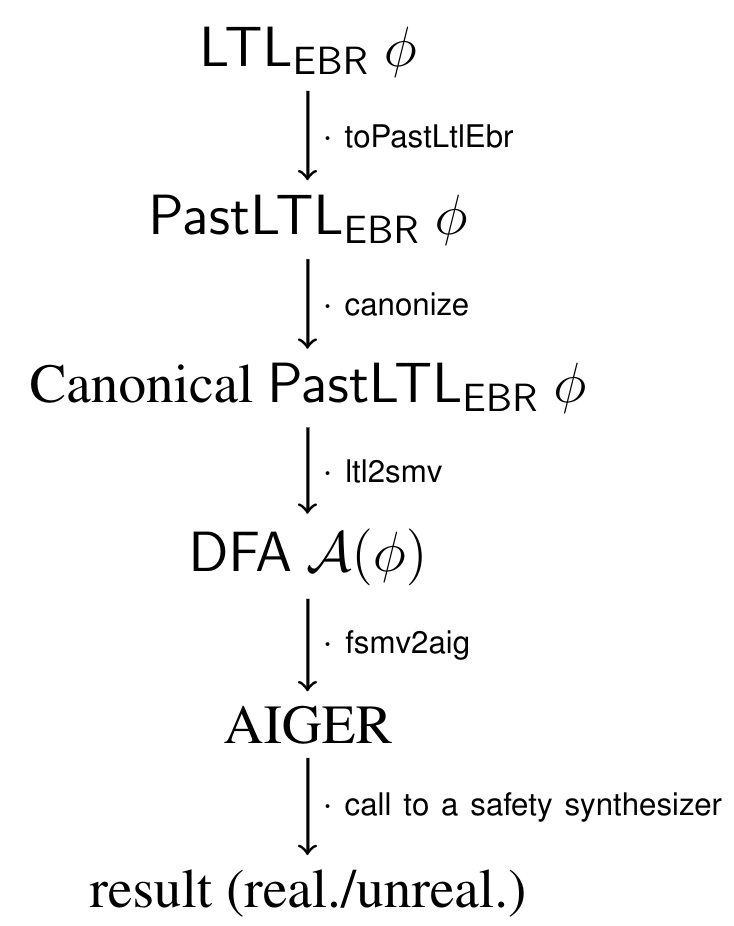
\includegraphics[width=0.4\linewidth]{figures/ebr-ltl-synthesis.png}
    \caption{\cite{geatti-2020-08} The overall procedure to synthesize a $\ebrltl$ formula}
    \label{fig:ebr-ltl-synthesis-procedure}
\end{figure}

The first step consists in translating each $\fpltl$ sub-formula in $\phi$ formula $\ebrltl$ into an equivalent one, which is of the form $\ltlXexp{\psi}{d}$, with $\psi \in \fpltl$ and $d \in \Nat$. This process is called pastification and is useful because full-past formulas can be represented by deterministic monitors, since "the past has already happened".

\begin{proposition}[\cite{geatti-2020-08} Soundness of pastification]
Let $\phi$ be a $\fbltl$ formula. For all state sequences $\sigma \in (2^\Sigma)^\omega$, all $i \in \Nat$ and all $d \geq D(\phi)$, it holds that
\begin{flalign*}
\sigma,i \models \phi \iff \sigma,i \models \ltlXexp{\Pi(\phi,d)}{d}
\end{flalign*}
\end{proposition}

The second step is the canonization of the $Past\ebrltl$ formula obtained from the previous step, in order to obtain an equivalent formula in canonical form. 
Canonical $Past\ebrltl$ formulas are Boolean combinations of formulas of the form $\ltlXexp{\psi_1}{i}$, $\ltlXexp{\ltlG{\psi_1}}{i}$, $\ltlXexp{\ltlR{\psi_1}{\psi_2}}{i}$, where $\psi_1$ and $\psi_2$ are full past formulas. 
Compared to general $Past\ebrltl$ formulas, formulas in canonical form do not admit neither nested unbounded operators nor next operators in front of the left-hand argument of a \textit{release}. The canonization of a $Past\ebrltl$ formula is obtained by applying a set of rewriting rules.
The particular shape of canonical $Past\ebrltl$ formulas makes it possible to encode the specifications into deterministic SSAs. The key observation is that $\fpltl$ formulas can be encoded into deterministic automata since these formulas exclusively talk about the past and so their truth can be evaluated at any single step depending only on previous steps, without making any guess about the future.

$Past\ebrltl$ in its canonical form combines full past formulas into a broader language that can still be turned into symbolic deterministic automata, exploiting the monitorability of universal temporal operators.
Consider the formula $\ltlG{\alpha}$. By observing a state sequence, at each step we can decide if a violation has occurred; indeed, if $\alpha$ is false at the current step, then the value of $\ltlG{\alpha}$ is certainly false for each of the previous steps. More generally, universal temporal formulas, such as $\ltlG{\alpha}$ and $\ltlR{\phi_1}{\phi_2}$, are monitorable, meaning that a violation of them can be decided on the basis of the observation of a finite number of steps. 
In particular, reporting an error in the next state can be done by considering only the current values. This means that any universal temporal operator can be monitored by adding a Boolean error variable with a deterministic transition relation. 
Therefore, despite not being able to evaluate the truth of a formula such as $\ltlG{\alpha}$, as it can be done in the case of past operators, we can nevertheless state in the accepting condition that an error state can never be reached. 
In this way, if the trace is accepting, that is an error state can never be reached, then we know that there are no violations, e.g., for $\ltlG{\alpha}$ we have forced $\alpha$ to be true in every state. 
Otherwise, if the trace is not accepting, that is an error state is reachable, we know that there is a (finite) violation and that the temporal formula was falsified at some step.
Therefore, we introduce an \textit{error bit} for each $\ltlXexp{\psi_1}{i}$, $\ltlXexp{\ltlG{\psi_1}}{i}$, $\ltlXexp{\ltlR{\psi_1}{\psi_2}}{i}$ of a canonical $Past\ebrltl$ formula.

Let $\phi$ be a canonical $Past\ebrltl$ formula over the alphabet $\Sigma = \C \cup \U$. We define the deterministic SSA $\automaton(\phi) = \tuple{V,I,T,S}$ as follows:
\begin{itemize}
    \item Variables. The set of state variables of the automaton is defined as $X = X_P \cup X_F \cup X_C$, where variables in $X_P$ track the truth value of all the full-past sub-formulas, variables in $X_F$ implement the monitoring mechanism and variables in $X_C$ are used to encode a binary counter used to monitor nested tomorrow operators. In particular, for $n$ nested tomorrow operators, a counter with $\log_2(n)$ bits is needed;
    \begin{flalign*}
        & X_P = \set{ \nu_\alpha \; | \; \text{$\alpha$ is a $\fpltl$ sub-formula of $\phi$}} \\
        & X_F = \set{error_\psi \; | \; \text{$\psi$ is a sub-formula of $\phi$ of the form $\ltlXexp{\psi}{i}$, $\ltlXexp{\ltlG{\psi}}{i}$ or $\ltlXexp{(\ltlR{\psi_1}{\psi_2})}{i}$}} \\
        & X_C = \set{counter_i \; | \; i \in \set{0,\dots,\log_2{d}} \text{with $d$ max. among all $X^d$ in $\phi$}}
    \end{flalign*}
    \item Initial state. All the state variables, including the counter bits, are initially false, that is $I(X) = \bigwedge_{x \in X} \ltlNeg{x}$;
    \item Transition relation. It is the conjunction of the transition functions of the binary counter and the monitors of each sub-formula of $\phi$.
    \item Safety condition. $S(X)$ is a Boolean formula obtained from $\phi$ by replacing each formula $\psi \in X_F$ by $\ltlNeg{error_\psi}$, i.e. $S(X) = \phi[\psi/\ltlNeg{error_\psi}]$.
\end{itemize}

We now define the monitors for the binary counter, used to handle nested \textit{tomorrow operators}, any formula $\psi \in \fpltl$ and any canonical $Past\ebrltl$. The monitor for the counter is defined as follows:
\begin{lstlisting}[language=smv, mathescape=true, caption=$\ebrltl$: counter]
next($counter_0$) := ($\bigwedge_{i=0}^n counter_i$) | $\neg counter_0$
next($counter_i$) := ($\bigwedge_{i=0}^n counter_i$) | (($counter_{i-1}$ | $counter_i$) & $\neg counter_i$)
\end{lstlisting}

If $\psi = \ltlS{\alpha}{\beta}$ or $\ltlY{\alpha}$, its monitor is defined as follows:
\begin{lstlisting}[language=smv,mathescape=true, caption=$\ebrltl$: yesterdat monitor]
next($\nu_{\ltlY{\alpha}}$) := $\nu_{\alpha}$
\end{lstlisting}
\begin{lstlisting}[language=smv,mathescape=true, caption=$\ebrltl$: since monitor]
DEFINE
    $\nu_{\ltlS{\alpha}{\beta}}$ := $\nu_\beta$ | ($\nu_\alpha$ & $\nu_{\ltlY{(\ltlS{\alpha}{\beta})}}$)
\end{lstlisting}

If $\psi$ is a propositional atom, a negation or a disjunction of full-past formulas, we define its monitor as follows:
\begin{lstlisting}[language=smv,mathescape=true, caption={$\ebrltl$: propositional atom, negation and disjunction monitors}]
DEFINE
    $\nu_p$ := $p$
    $\nu_{\ltlNeg{\alpha}}$ := !$\nu_\alpha$
    $\nu_{\ltlOr{\alpha}{\beta}}$ := $\nu_{\alpha}$ | $\nu_{\beta}$
\end{lstlisting}

For each formula $\phi$ of type $\ltlXexp{\psi}{i}$, where $\psi$ is a full-past formula, we introduce a new error bit $error_\phi$. Its monitor is defined as follows:
\begin{lstlisting}[language=smv,mathescape=true, caption=$\ebrltl$: next of proposition monitor]
next($error_{\ltlXexp{\psi}{i}}$) := case
    $error_{\ltlXexp{\psi}{i}}$ : TRUE;
    counter = i & !$\nu_{\psi}$ : TRUE;
    TRUE : FALSE;
  esac;
\end{lstlisting}

If $\phi = \ltlXexp{\ltlG{\psi}}{i}$, where $\psi$ is a full-past formula, we introduce a new error bit $error_\phi$ and define its monitor as follows:
\begin{lstlisting}[language=smv, mathescape=true, caption=$\ebrltl$: next of globally monitor]
next($error_{\ltlXexp{\ltlG{\psi}}{i}}$) := case
    counter < i : FALSE;
    !$error_{\ltlXexp{\ltlG{\psi}}{i}}$ & $\nu_{\psi}$ : FALSE;
    TRUE : TRUE;
  esac;
\end{lstlisting}

The same for $\phi = \ltlXexp{\ltlR{\psi_1}{\psi_2}}{i}$:
\begin{lstlisting}[language=smv, mathescape=true, caption=$\ebrltl$: next of release monitor]
next($error_{\ltlXexp{\ltlR{\psi_1}{\psi_2}}{i}}$) := case
    counter < i : FALSE;
    !$error_{\ltlXexp{\ltlR{\psi_1}{\psi_2}}{i}}$ & $\nu_{\psi_1^p}^i$ : FALSE;
    !$error_{\ltlXexp{\ltlR{\psi_1}{\psi_2}}{i}}$ & $\nu_{\psi_1}$ & $\nu_{\psi_2}$ : FALSE;
    !$error_{\ltlXexp{\ltlR{\psi_1}{\psi_2}}{i}}$ & $\nu_{\psi_2}$ : FALSE;
    TRUE : TRUE;
  esac;

next($\nu_{\psi_1^p}^i$) := case
    counter < i : FALSE;
    $\nu_{\psi_1^p}$ : TRUE;
    $\nu_{\psi_1^p}^i$ : TRUE;
    TRUE : FALSE;
  esac;
\end{lstlisting}

Moreover, we define two further monitors which are useful in the next chapter since, even though they are not defined in \cite{geatti-2020-08}.
The monitors are those for trigger and conjunction operators.
If $\phi = \ltlT{\alpha}{\beta}$ or $\phi = \ltlAnd{\alpha}{\beta}$, the monitors for such formulas can be defined as follows:
\begin{lstlisting}[language=smv, mathescape=true, caption=$\ebrltl$: trigger monitor]
DEFINE
    $\nu_{\ltlT{\alpha}{\beta}}$ := $\nu_\beta$ & ($\nu_\alpha$ | $\nu_{\ltlT{\alpha}{\beta}}$)
\end{lstlisting}
\begin{lstlisting}[language=smv, mathescape=true, caption=$\ebrltl$: conjunction monitor]
DEFINE
    $\nu_{\ltlAnd{\alpha}{\beta}}$ := $\nu_{\alpha}$ & $\nu_{\beta}$
\end{lstlisting}


\begin{figure}[!htp]
    \centering
    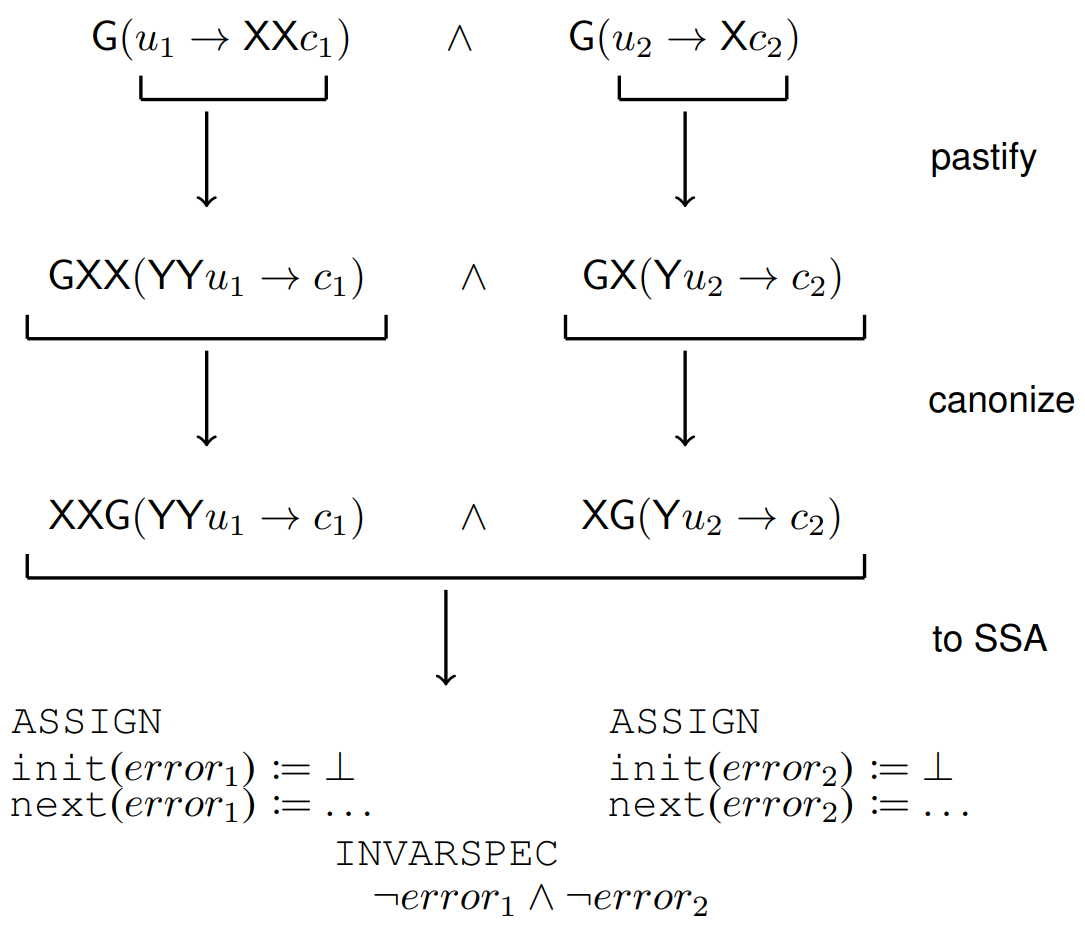
\includegraphics[width=0.6\linewidth]{figures/ebr-ltl-synthesis-example.png}
    \caption{\cite{geatti-2020-08} Example of $\ebrltl$ synthesis for the formula $\ltlAnd{\ltlG{(u_1 \to \ltlX{\ltlX{c_1}})}}{\ltlG{(u_2 \to \ltlX{c_2})}}$}
    \label{fig:ebr-ltl-synthesis-example}
\end{figure}

After having built the automaton, the respective safety game $\game = \tuple{\automaton_\phi, \C, \U}$ is converted to AIGER format and then given as input to the chosen safety synthesizer, completing the process described previously. It has been proved that the overall procedure belongs to $2EXPTIME$ complexity class, while it belongs to $EXPTIME$ if no constants are admitted managing to get rid of an exponential.

\begin{proposition}[\cite{geatti-2020-08} $\ebrltl$ synthesis complexity]
The realizability problem for $\ebrltl$ belongs to $2EXPTIME$. 
If no constant is admitted, it belongs to $EXPTIME$.
\end{proposition}

The $\ebrltl$ synthesis procedure is implemented in nuXmv under the command \lstinline{_ebr2fsmv}, which reads in input a $\ebrltl$ formula and produces the deterministic SSA of such formula. The SSA is represented by functional SMV modules, that is SMV modules characterized by only Boolean state variables and initial states and next transitions defined via \lstinline{init(var)} and \lstinline{next(var)} statements.
The conversion of SSAs from functional SMV to AIGER format is performed by the command \lstinline{fsmv2aig} implemeted in nuXmv.


